\chapter{Cardea}\label{sec-cardea}

\section{System Design}
Recalling related works in Chapter 2, what motivates the design of Cardea are the follow:

\begin{itemize}
\item People's privacy concerns are dependent on context. Although in certain circumstances locations are strong hints of possible privacy intrusion, generally what individuals are doing and with whom are more essential and crucial factors that directly relate to privacy.
\item People's privacy preferences vary from each other, thus they should be able to express their personal privacy preferences.
\item People's privacy preferences may change from time to time, therefore they need a way to change such preferences easily.
\end{itemize}

To achieve these objectives, we propose following solution:
\begin{itemize}
  \item We combine GPS location, grouped scene categories (Table~\ref{tbl-scenecate}) and accompanied persons as context that can better represent people's privacy concerns than previous methods. As a result we are able to provide more general as well as finer granularity privacy preference settings for users.
\item We use cloud server to host individualized privacy preferences, and user's preference is binded with his facial features. In this way his raw visual information stays locally, preventing the case of visual privacy leakage from hacked servers.
\item Other than a simple interface provided to users to update their privacy preferences, hand gestures like \vcenteredinclude{figure/ch4-yesgesticon.png} and \vcenteredinclude{figure/ch4-nogesticon.png} can be used by user to actively speak out about his preference in the capturing moment, enriching the interaction and adding more flexibilities.
\end{itemize}
As introduced in chapter 3, breakthroughs made by deep learning community in many computer vision problems such as image classification, face recognition and object detection have guided the proposed solution and shed lights on its practicability. More specifically, given a captured image, Cardea will leverage powerful convolutional neural networks to for the recognition of scene context, registered users and gestures. Cardea's design is given in Fig~\ref{fig:ch4-cardeadesign}, it is composed of the client applications and cloud server. It works based on data exchange and collaborative computing involving both client and cloud sides. The major components and interactions include:
\begin{figure}[!htbp]
    \centering
    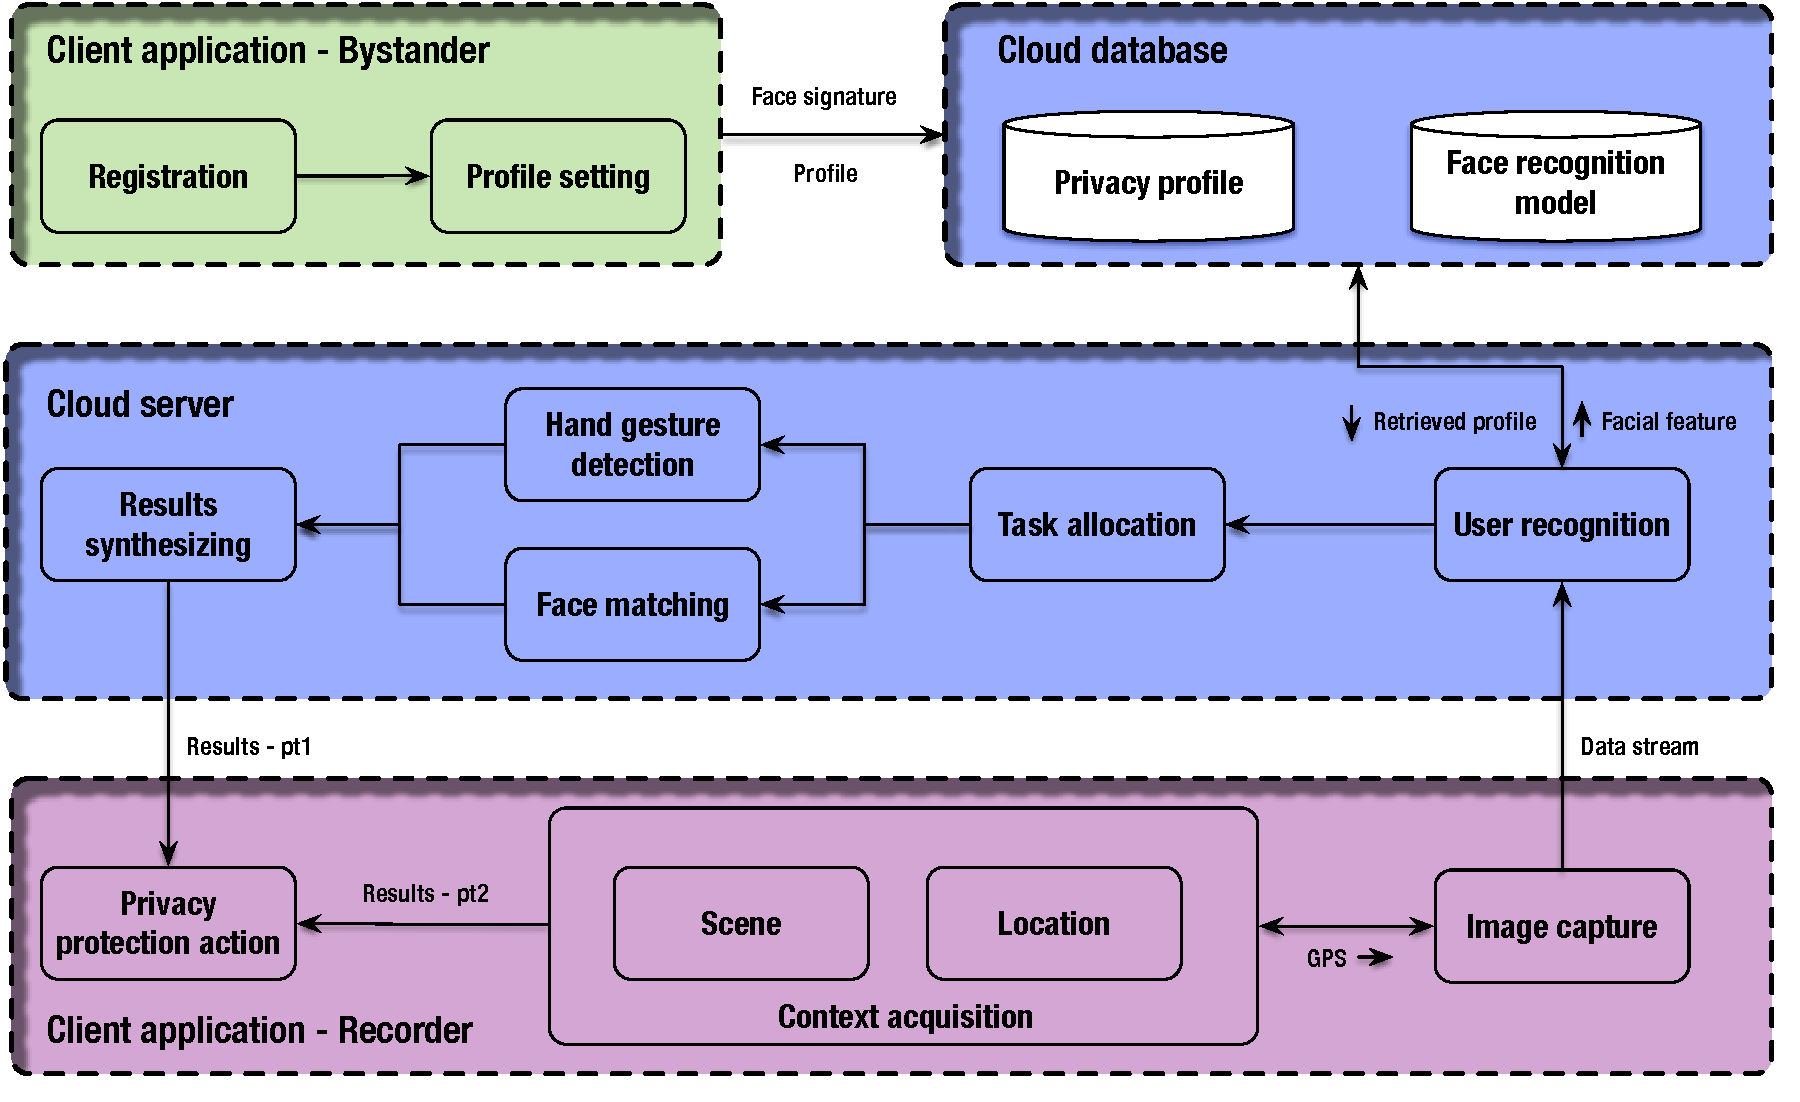
\includegraphics[width=1.0\textwidth]{figure/ch4-cardeadesign.pdf}
    \caption{System design of Cardea.}
    \label{fig:ch4-cardeadesign}
\end{figure}

\begin{description}[leftmargin=0cm]
  \item[{\bfseries Bystander client application:}] A bystander can use this application to register as Cardea user and define his privacy profile. It will capture a number of face images (about 50–60 images) and extract facial features from these images as his unique face signature. After setting up the context dependant privacy preference, his facial signature and preference will be sent to cloud server for registration and updating of face recognition model.
  \item[{\bfseries Recorder client application:}] A recorder can use this application to take images that will automatically perform privacy protection actions in compliance with all Cardea users' privacy preferences. Given a captured image, it first detects all the faces and extracts the corresponding facial features locally on device, then the features and the captured image but is compressed and with all detected faces blurred are sent to the server for face and gesture recognitions. GPS coordinate is also sent to server in this step to be compared with recognized users' location settings. During the time waiting for response from cloud, it performs scene group prediction task. Finally, predicted scene group and intermediate decision result received from server are used to decide the actual protection action which will be enforced on the raw captured image.
  \item[{\bfseries Cloud server:}] The cloud server serves as two roles: \ding{182} When receives requests from Bystander applications, it will store/update users' profiles, and training/updating system's face recognition model automatically; \ding{183} When receive requests from Recorder applications, it will initiate face and gesture recognition tasks, as well as partial decision making based on recognition results, and send these intermediate decision results to client for final step of decision making.
\end{description}

Implementations of each module, how Cardea allocates tasks between mobile and cloud, integration, usage and performance evaluation of the whole system are discussed throughly in following sections.

\begin{table}[tb]
\centering
\caption{Scene categories.}
\label{tbl-scenecate}
\begin{tabular}{ll}
\toprule
Scene Group    & Scene Category                                       \\ \midrule
Eating         & bistro/indoor, bistro/outdoor, cafeteria, coffee\_shop, \\
               & diner/outdoor, dining\_hall, dining\_room, fastfood\_restaurant, food\_court, \\
               & restaurant, restaurant\_patio, sushi\_bar            \\ \midrule
Entertainment  & bar, discotheque, pub/indoor                         \\ \midrule
Shopping       & bazaar/indoor, bazaar/outdoor, clothing\_store, general\_store/indoor, \\
               & jewelry\_shop, shoe\_shop, shopping\_mall/indoor, supermarket  \\ \midrule
Work           & conference\_center, conference\_room, cubicle/office, library/indoor, office, \\
               & office\_cubicles, reading\_room                      \\ \midrule
Public         & park, street                                         \\ \midrule
Mobility       & airplane\_cabin, airport\_terminal, bus\_interior, bus\_station/indoor, \\
               & subway\_station/platform, train\_interior, train\_station/platform \\ \midrule
Exhibition     & art\_gallery, museum/indoor                          \\ \midrule
Religion       & cathedral/indoor, cathedral/outdoor, church/indoor, church/outdoor, mosque/outdoor, \\
               & pulpit, temple/east\_asia, temple/south\_asia        \\ \midrule
Illness        & hospital, hospital\_room, nursing\_home                \\ \midrule
Nudity         & bathroom, beach, jacuzzi/indoor, sauna, shower, \\
               & swimming\_pool/indoor, swimming\_pool/outdoor        \\ \bottomrule
\end{tabular}
\end{table}




\section{Implementation}

\subsection{Scene Classification}

\subsubsection{Data Preparing and Preprocessing}

For scene classification, we use pre-trained model of Places2 dataset provided by~\cite{links:places2mit}. In the time Cardea project was conducted, Places2 dataset provided by the authors contained 401 categories with more than 8 million training images, and the pre-trained model was based on AlexNet structure~\cite{krizhevsky2012imagenet}. By the time this thesis is writing, the dataset is deprecated and the new Places2 dataset contains 365 categories. And the authors provide more pre-trained models based on different network structures~\cite{links:places2pre}.

\begin{figure}[!htbp]
    \centering
    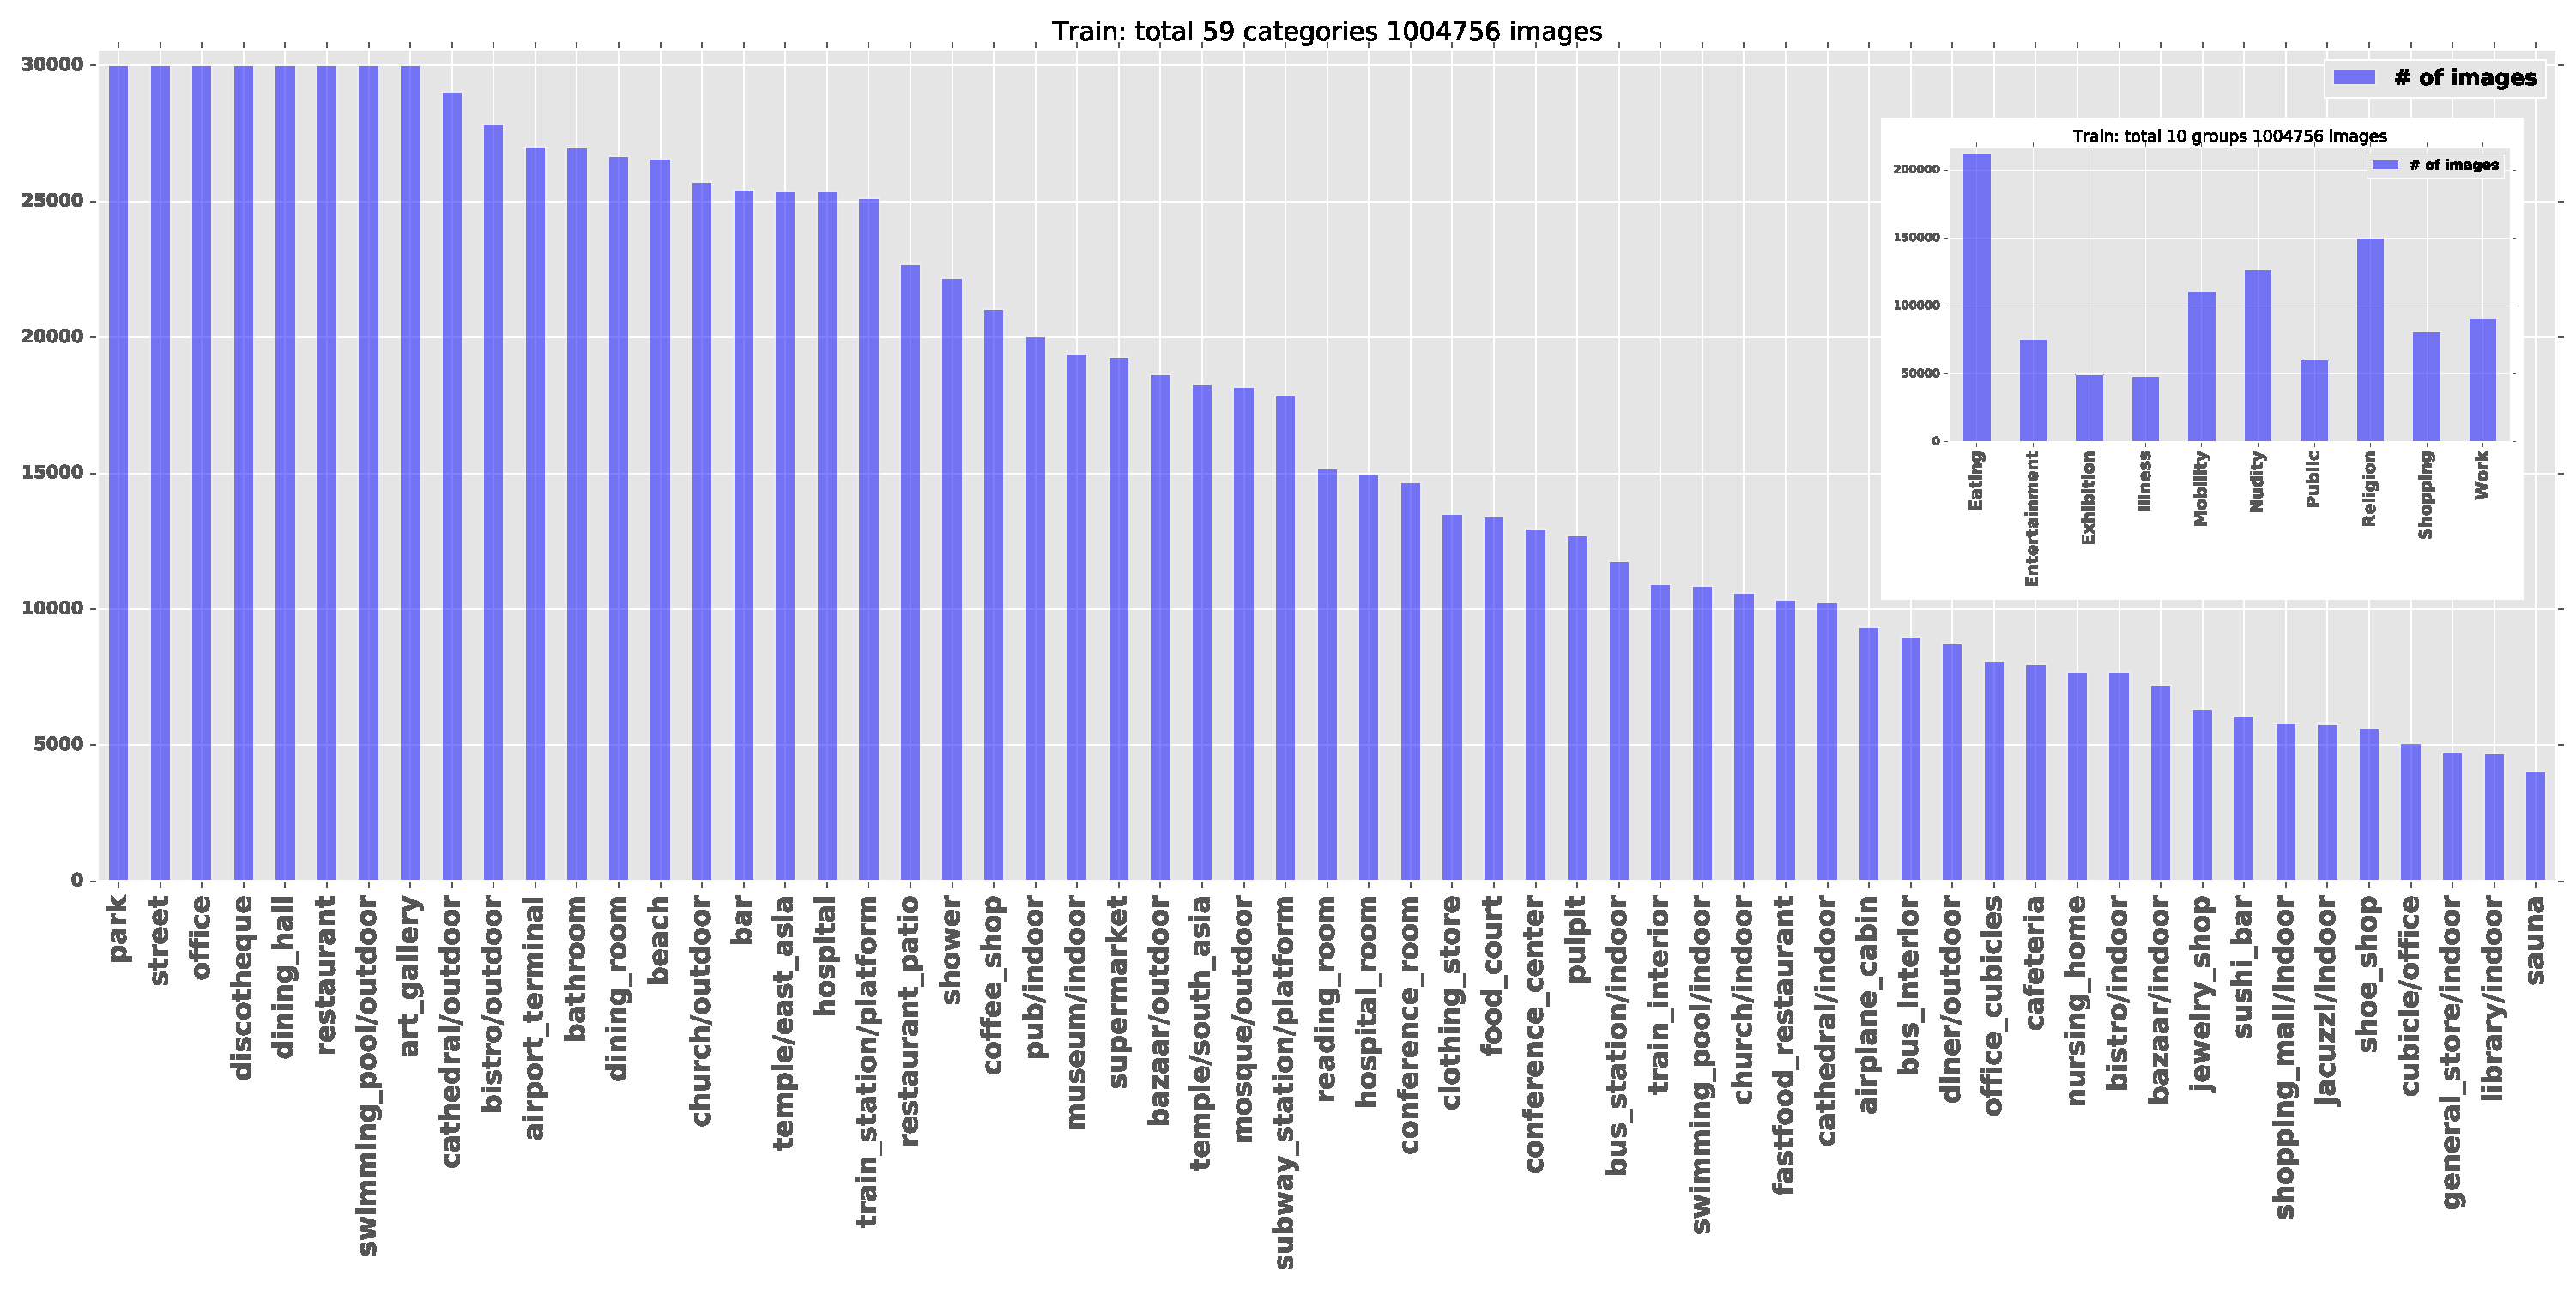
\includegraphics[width=1.0\textwidth]{figure/ch4-numdist.pdf}
    \caption{Number of images for each category and each group (inset).}
    \label{fig:ch4-scenenumdist}
\end{figure}

Note that in the dataset we used, there is a non-uniform distribution of images per category for training, ranging from 4,000 to 30,000, mimicking a more natural frequency of occurrence of the scene. Among the 401 categories, we choose 59 scene categories that are close to daily life and in such scenes people may have privacy concern. In total this subset composed of 1 million training images and 2950 validation images (50 validation images for each category). We also group these 59 scene categories into 10 groups based on contextual similarity as shown in Table~\ref{tbl-scenecate}, such that people have similar reasons for privacy in scenes that are in the same group (e.g. people don't want to be captured in bathroom and beach is both because of nudity concerns). The distribution of training images among categories and groups is shown in Fig~\ref{fig:ch4-scenenumdist}.

\subsubsection{Training Procedures}
Our training step is just a standard fine-tuning process, which is extensively used in transfer learning~\cite{sharif2014cnn,yosinski2014transferable}:

\begin{itemize}
\item[\ding{182}] Using pre-trained model as feature extractor, we extract the features at \emph{fc7} layer for images belonging to the 59 picked categories. Other than shuffling the features, we also augment the features such that all categories have same amount of features. Though the natural frequencies of occurrence are obviously different among different scenes, we argue that for the purpose of privacy protection, all the scene categories should be equally important, thus categories imbalance is not what we favored. The augmentation step can be implemented using weighted loss layer, but we take simple way of bootstrapping features for categories with less images. After this step, all features are cached and stored in lmdb format.
\item[\ding{183}] Train a softmax classifier of the 59 categories using the extracted features. We choose to train a classifier for categories and then add up the output probabilities to predict the group, rather than directly train a group classifier, is because category classifier tells more about the image, and our desired property is equal weights among scene categories rather than groups.
\item[\ding{184}] Both feature extraction and classifier training are implemented using Caffe library~\cite{links:caffelib,jia2014caffe}. In this step we merge the feature extraction part of pre-trained model and the softmax classifier into a single model by copying weights. Now Caffe has the option of specifying layers with fixed weights, thus simplifying the fine-tuning and deployment process.
\end{itemize}

Other than improving the validation accuracy from 0.56 to 0.57, shuffling also makes training converges faster. With augmentation to relieve category imbalance issue, the classifier can finally achieve 0.600 validation accuracy on the 59 categories. There is no other benchmarking result specifically on the subset we choose, but recent benchmark gives 53\%-56\% validation accuracy on the new Places2 dataset with 365 categories~\cite{links:places2pre}, suggesting our model is competitive. The higher validation accuracy of our model is due to the smaller scale of classification problem we are dealing with.

\subsubsection{Prediction}

\begin{figure}[!t]
    \centering
    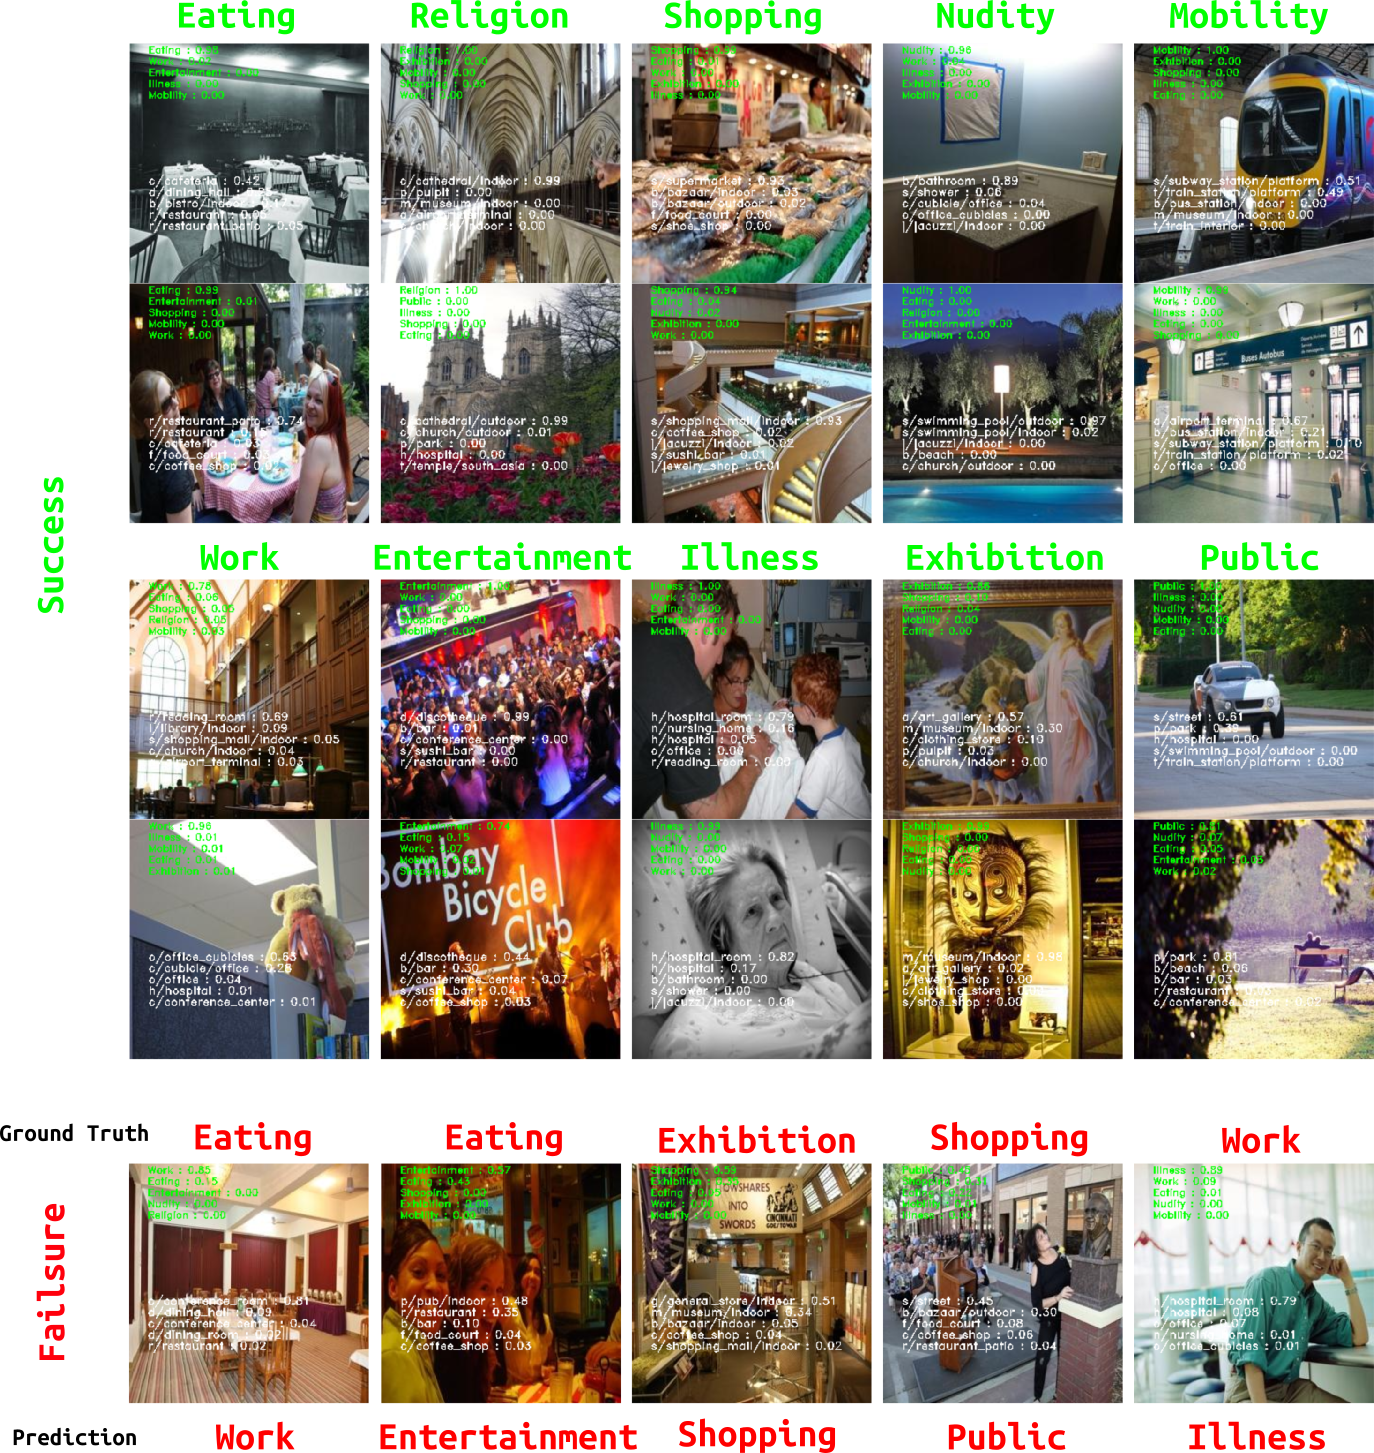
\includegraphics[width=\textwidth]{figure/ch4-scnpredictemp.png}
    \caption{Scene classification prediction example. Top5 groups (green) and categories (white) are shown with their probabilities.}
    \label{fig:ch4-scnpredictemp}
\end{figure}

For prediction, we get probability of a group by summing up the probabilities of all categories belonging to this group, and output the most probable group as prediction of an image. Our model's group prediction accuracy for the validation set is 82.8\%. Fig~\ref{fig:ch4-scnpredictemp} shows some prediction examples. As seen from the examples, given an image, the predicted category probabilities are usually stratified to few categories within same group, thus group prediction is resilient to perturbation of category prediction. The way we group categories can be seemed as a hard-coded clustering step, which makes prediction more robust to noise. The failure cases are mostly due to natural context ambiguity from a image (e.g. image with object in focus, therefore not enough hints for scene inference). Labeling the 342 non selected categories as extra group will amplify the ambiguity issue, even for images with less ambiguity, doing so will stratify probabilities to the extra group and lead to wrong prediction. In other words, a 59 way classifier leads to higher recall for selected scenes and grouping leads to higher accuracy. This is also reflected in confusion matrices shown in Fig~\ref{fig:ch4-scnconfumat}, category confusion matrix shows some clustering structure which is in accordance with the groups we manually assigned. However, only using top 1 category for prediction sacrifices prediction accuracy, which can be avoided by grouping as shown in group confusion matrix.

\begin{figure}[!htbp]
    \makebox[\textwidth]{
        \centering
        \raisebox{-0.5\height}{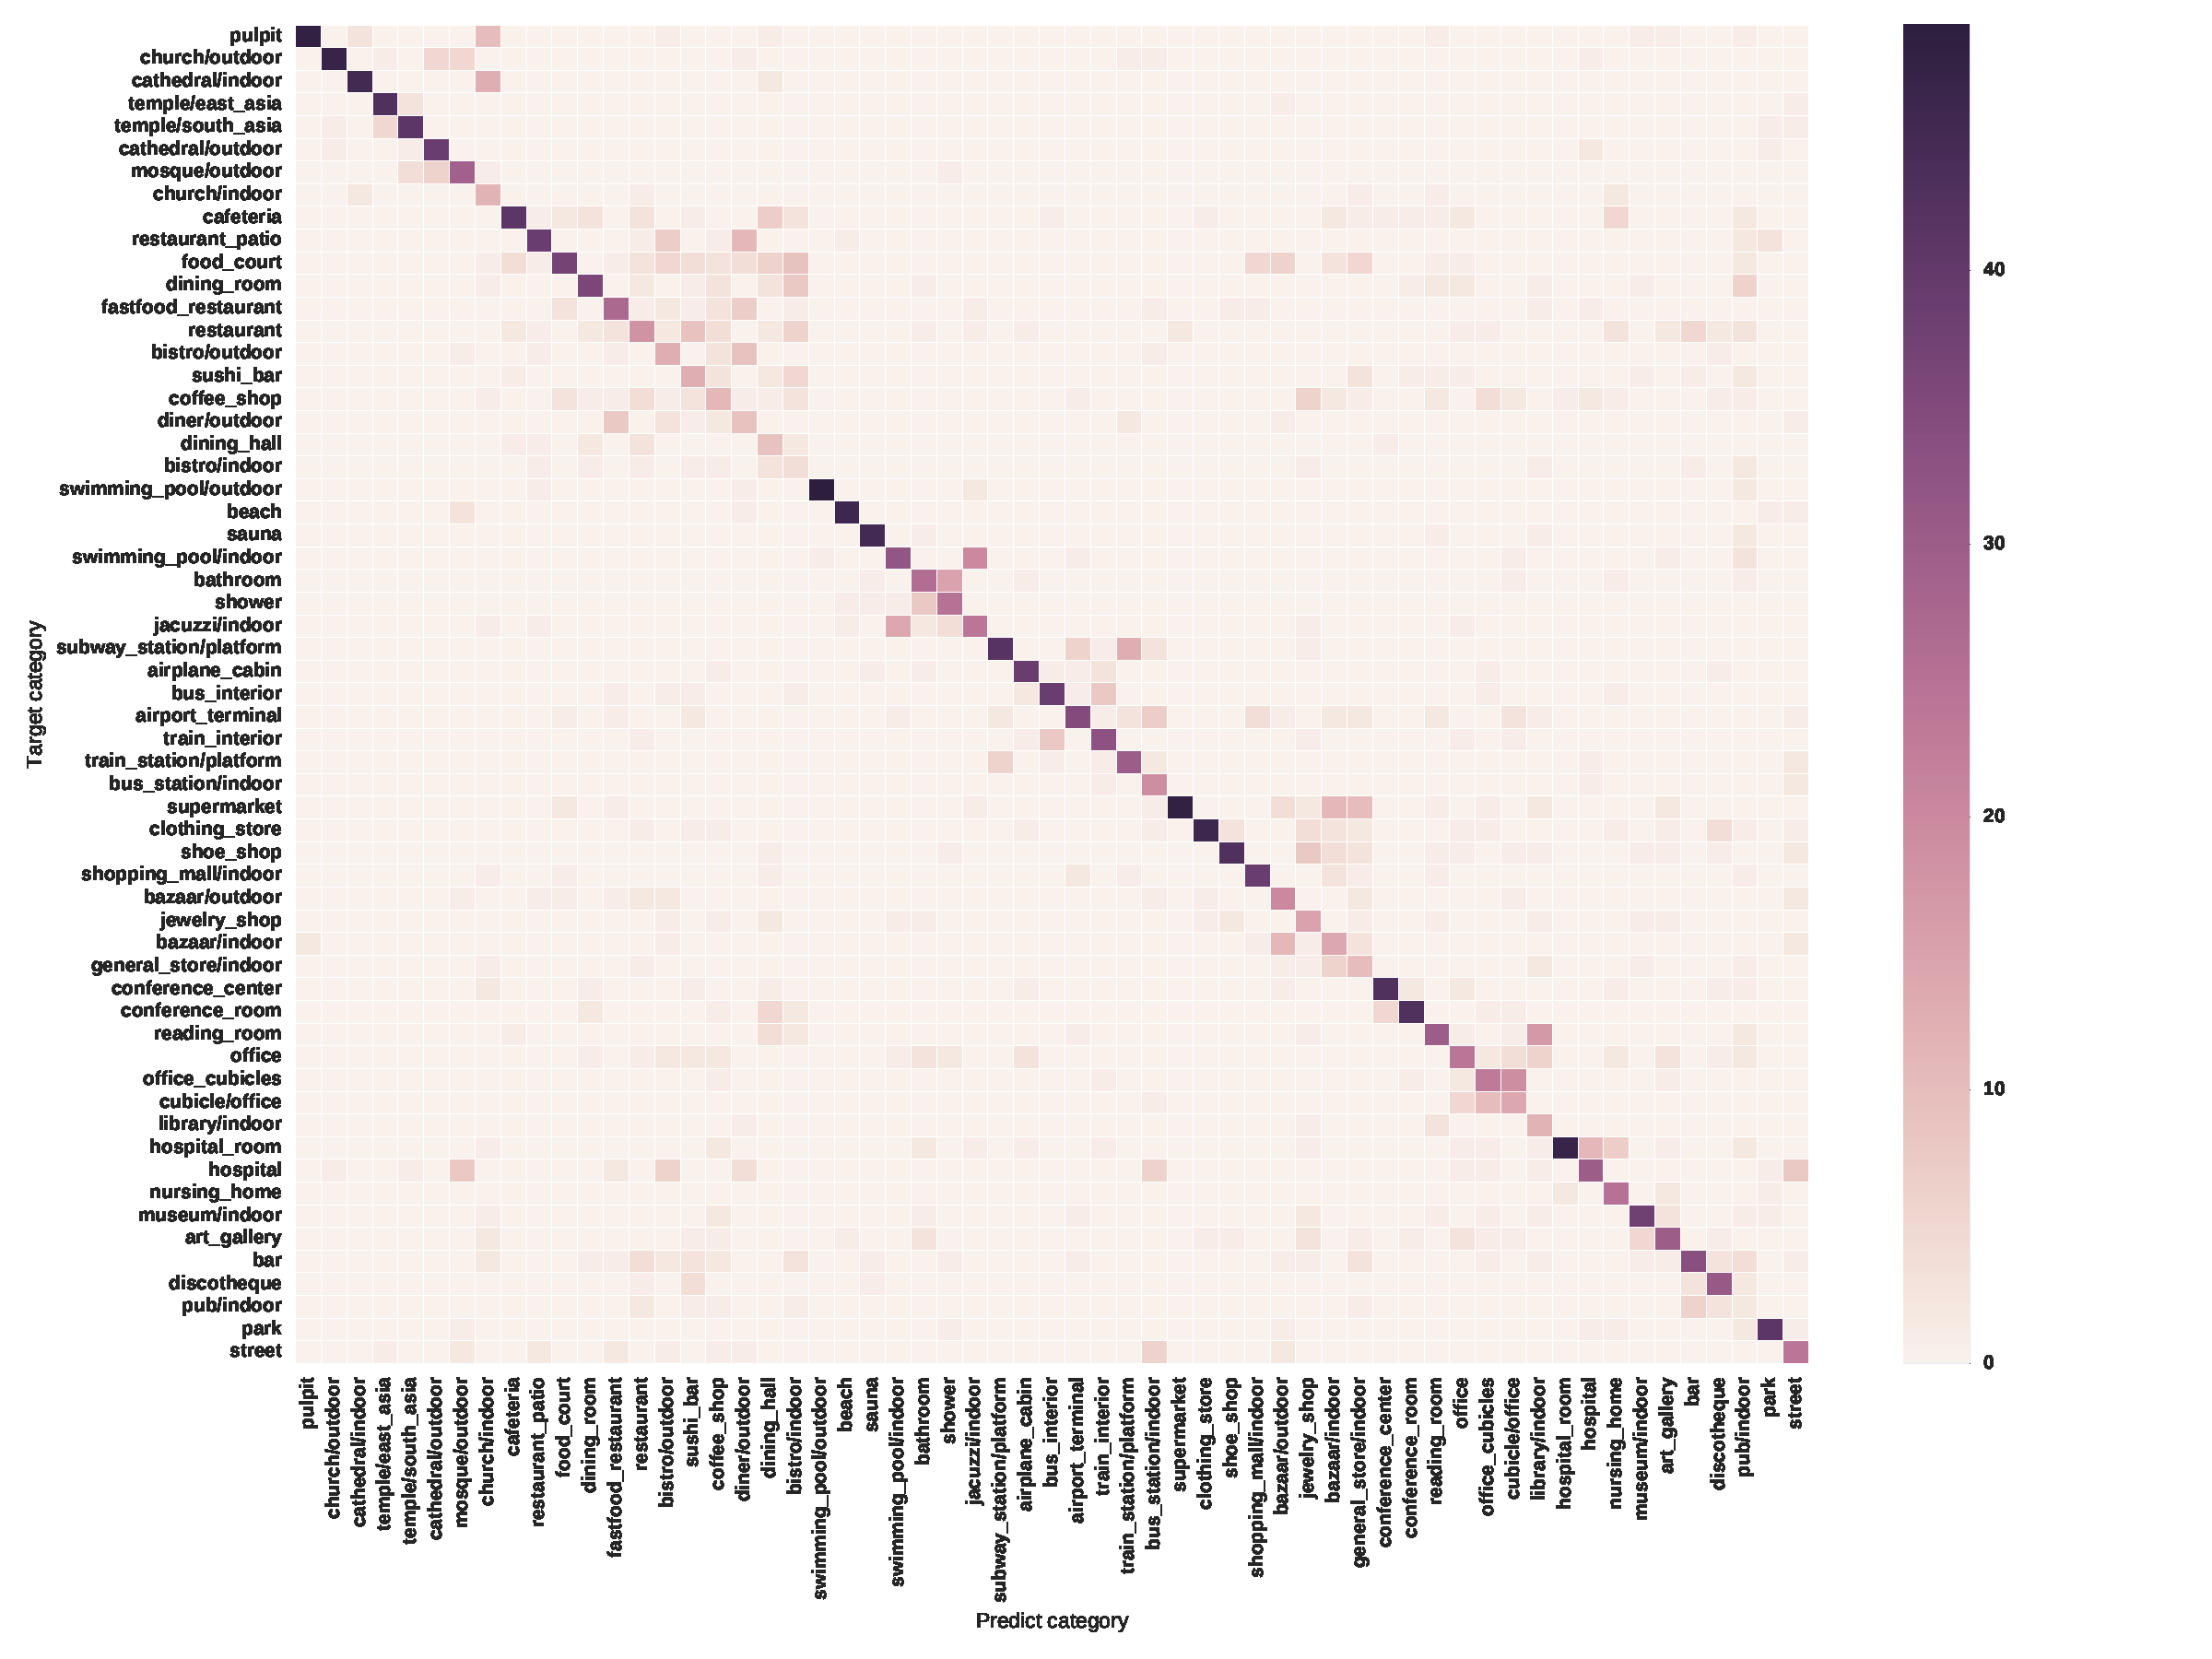
\includegraphics[width=0.7\textwidth]{figure/ch4-scnCateConfu.pdf}}
        \hspace{-1cm}%
        \raisebox{-0.5\height}{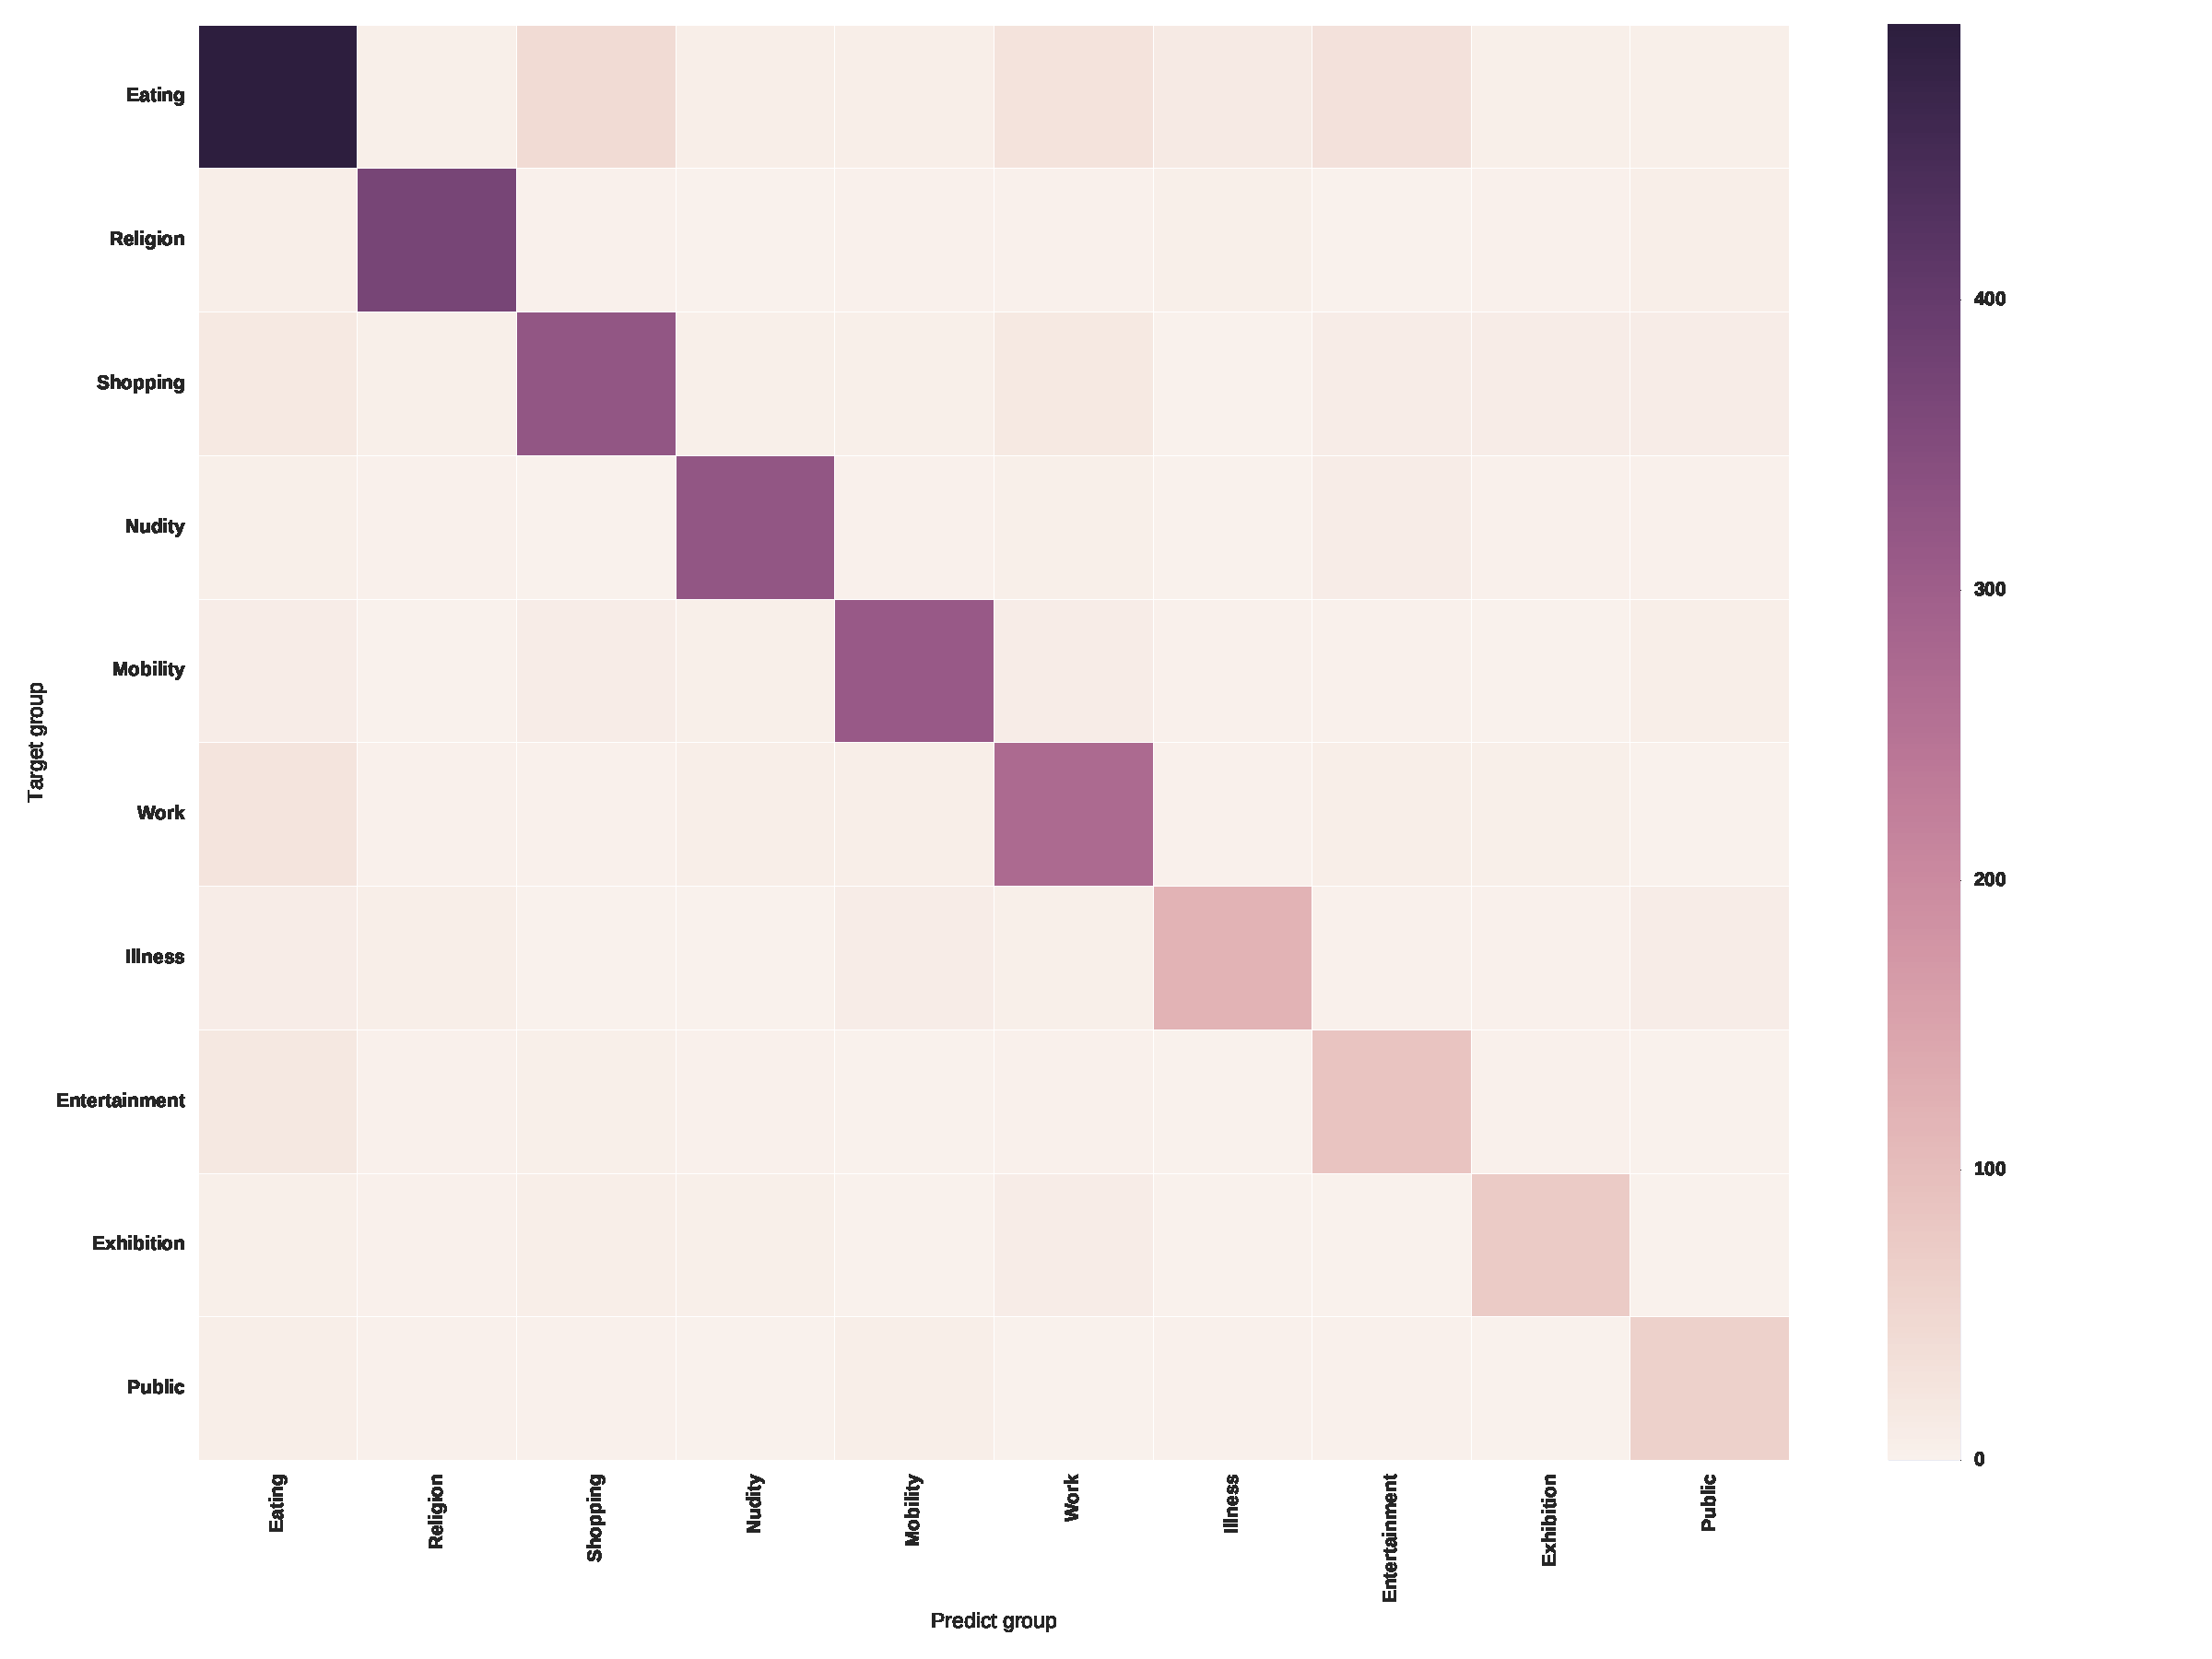
\includegraphics[width=0.6\textwidth]{figure/ch4-scnGrpConfu.pdf}}
    }
    \caption{Confusion matrices for category prediction (left) and group prediction (right).}
    \label{fig:ch4-scnconfumat}
\end{figure}



\subsection{Face Recognition}
Like scene classification, we select a pre-trained model for face recognition task. More specifically, the pre-trained model will serve as face feature extractor, and we will update the face classifier whenever new users register in Cardea and upload their face features. There are already many deep neural networks deployed in commercial products, like Megvii's Face++~\cite{zhou2013extensive}, Facebook's Deepface~\cite{taigman2014deepface}, Google's Facenet~\cite{schroff2015facenet}, Sensetime's Deepid~\cite{sun2015deepid3}. OpenFace~\cite{amos2016openface} is an open source project that is gaining attentions in recent months, it is based on Torch~\cite{links:torch7}. Because Cardea's other modules are under Caffe framework, we limit our options on open sourced Caffe models. The models in our consideration are VGG face recognition model~\cite{parkhi2015deep} and Lightened CNN face recognition model~\cite{wu2015lightened}.

\begin{figure}[!htbp]
    \makebox[\textwidth]{
        \centering
        \raisebox{-0.5\height}{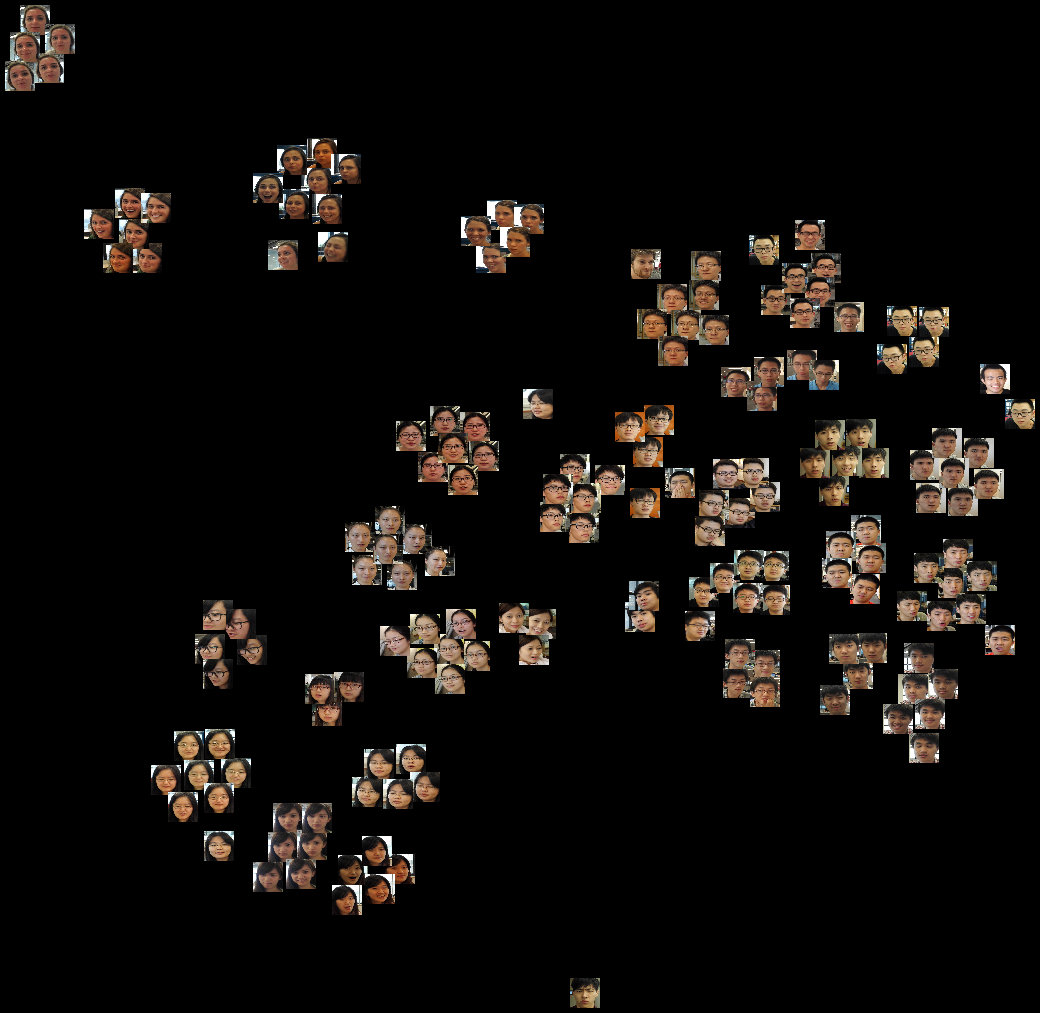
\includegraphics[width=0.6\textwidth]{figure/ch4-tsnevggfc8.png}}
        \raisebox{-0.5\height}{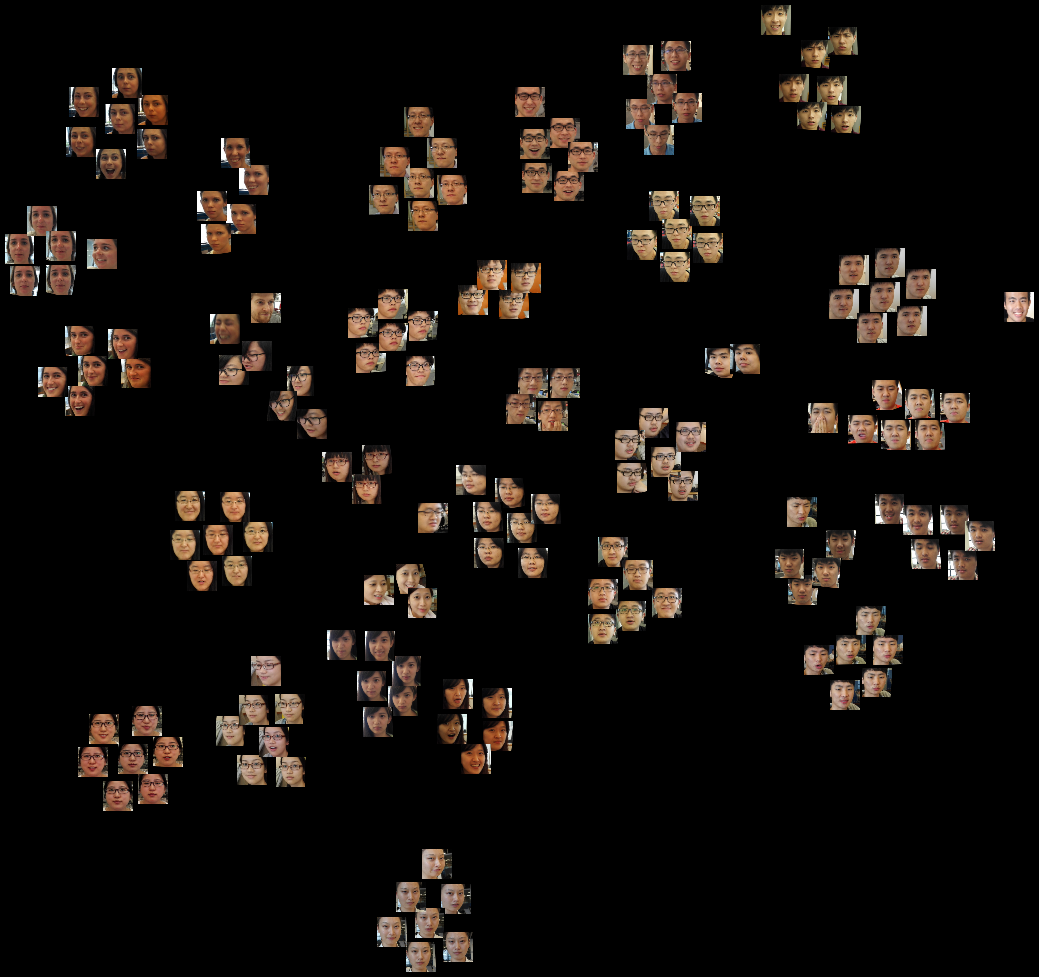
\includegraphics[width=0.62\textwidth]{figure/ch4-tsnemfmeltwise_fc1.png}}
    }
    \caption{t-SNE visualization of VGG \emph{fc8} layer features and Lightened CNN \emph{fc1} layer features.}
    \label{fig:ch4-tsnevggvsmfm}
\end{figure}

To compare performance of features extracted from the two models, we run t-SNE visualization~\cite{maaten2008visualizing} on the features of a small dataset we previously collected for emotion sensing. Fig~\ref{fig:ch4-tsnevggvsmfm} shows the t-SNE visualization result. It seems VGG feature and Lightened CNN feature have similar performance, at least on this small dataset. Though it is found that comparing to Lightened CNN model, VGG model is more robust to variations and its features show better transferability~\cite{ghazi2016comprehensive}, the model size is more than 500MB, 10 times bigger than Lightened CNN model. And the released VGG model has a feature dimension of 4096, while Lightened CNN model has a feature dimension of 256. Our experiment on different Android smartphones shows it takes 10 times longer to extract VGG features. Table~\ref{tbl-forwardingtime} shows the forwarding time we tested on different smartphones. It can be seen VGG model consumes much more memory that it can only run on phones with memory larger than 3GB. Due to above concerns, we use Lightened CNN model in our implementation.

\begin{table}[!htbp]
\centering
\caption{Time of single facial feature extraction and batch facial feature extraction (10 faces).}
\label{tbl-forwardingtime}
\begin{tabular}{lrrr}
\toprule
 & Xiaomi Mi 3W & Galaxy Note 4 & Xiaomi Mi 5\\
 & {\small Snapdragon 800} & {\small Snapdragon 805} & {\small Snapdragon 820}\\
 & {\small 2GB RAM} & {\small 3GB RAM} & {\small 4GB RAM}\\
 \midrule
1 VGG CNN & N/A & N/A & $\sim 2780$ ms \\
10 VGG CNN & N/A & N/A & $\sim 26740$ ms \\
1 Lightened CNN & $\sim 508$ ms & $\sim 330$ ms & $\sim 303$ ms \\
10 Lightened CNN & $\sim 6602$ ms & $\sim 3971$ ms & $\sim 2031$ ms \\
 \bottomrule

\end{tabular}
\end{table}


\subsubsection{Detection and Alignment}
Lightened CNN model takes aligned face as input, requiring that the distance between midpoint of eyes and midpoint of mouth is 48, and $y$ value of midpoint of eyes is 40, as shown in Fig~\ref{fig:ch4-facedetalign}. We use OpenCV's haar cascade~\cite{links:opencv,viola2001rapid} frontal face detector. The limitation it brings to Cardea is only frontal faces will be detected and recognized. We set \emph{minNeighbors} (the parameter specifying how many neighbors each candidate rectangle should have to retain it) to be 3 to ensure a relative high recall for face detection. To remove false positive, we further apply skin color filter (range $[0, 48, 60] - [30, 255, 255]$ in HSV color space) on retained rectangles. Following that, we use Dlib library's HOG~\cite{links:dlib,dalal2005histograms} based face detector as a second stage filter. Note that Dlib's face detector has higher accuracy comparing to OpenCV's face detector, but is much slower if applied directly on a high resolution image, therefore it is used as a filter on small rectangular areas. Dlib's facial landmarks detector~\cite{links:dlibfacepose} is also used in later face alignment stage, it can detect 68 facial landmarks~\cite{links:dlibfacelandmarkspos, links:dlibfacelandmarkscoords}. With the detected landmarks and required alignment condition about inputs to the CNN model, we can calculate the homography matrix that is finally used to align faces. The steps for detection and alignment is shown in Fig~\ref{fig:ch4-facedetalign}, and we implemented it as a JNI library for Android platform~\cite{links:facealignjni}.

\begin{figure}[!htbp]
    \centering
    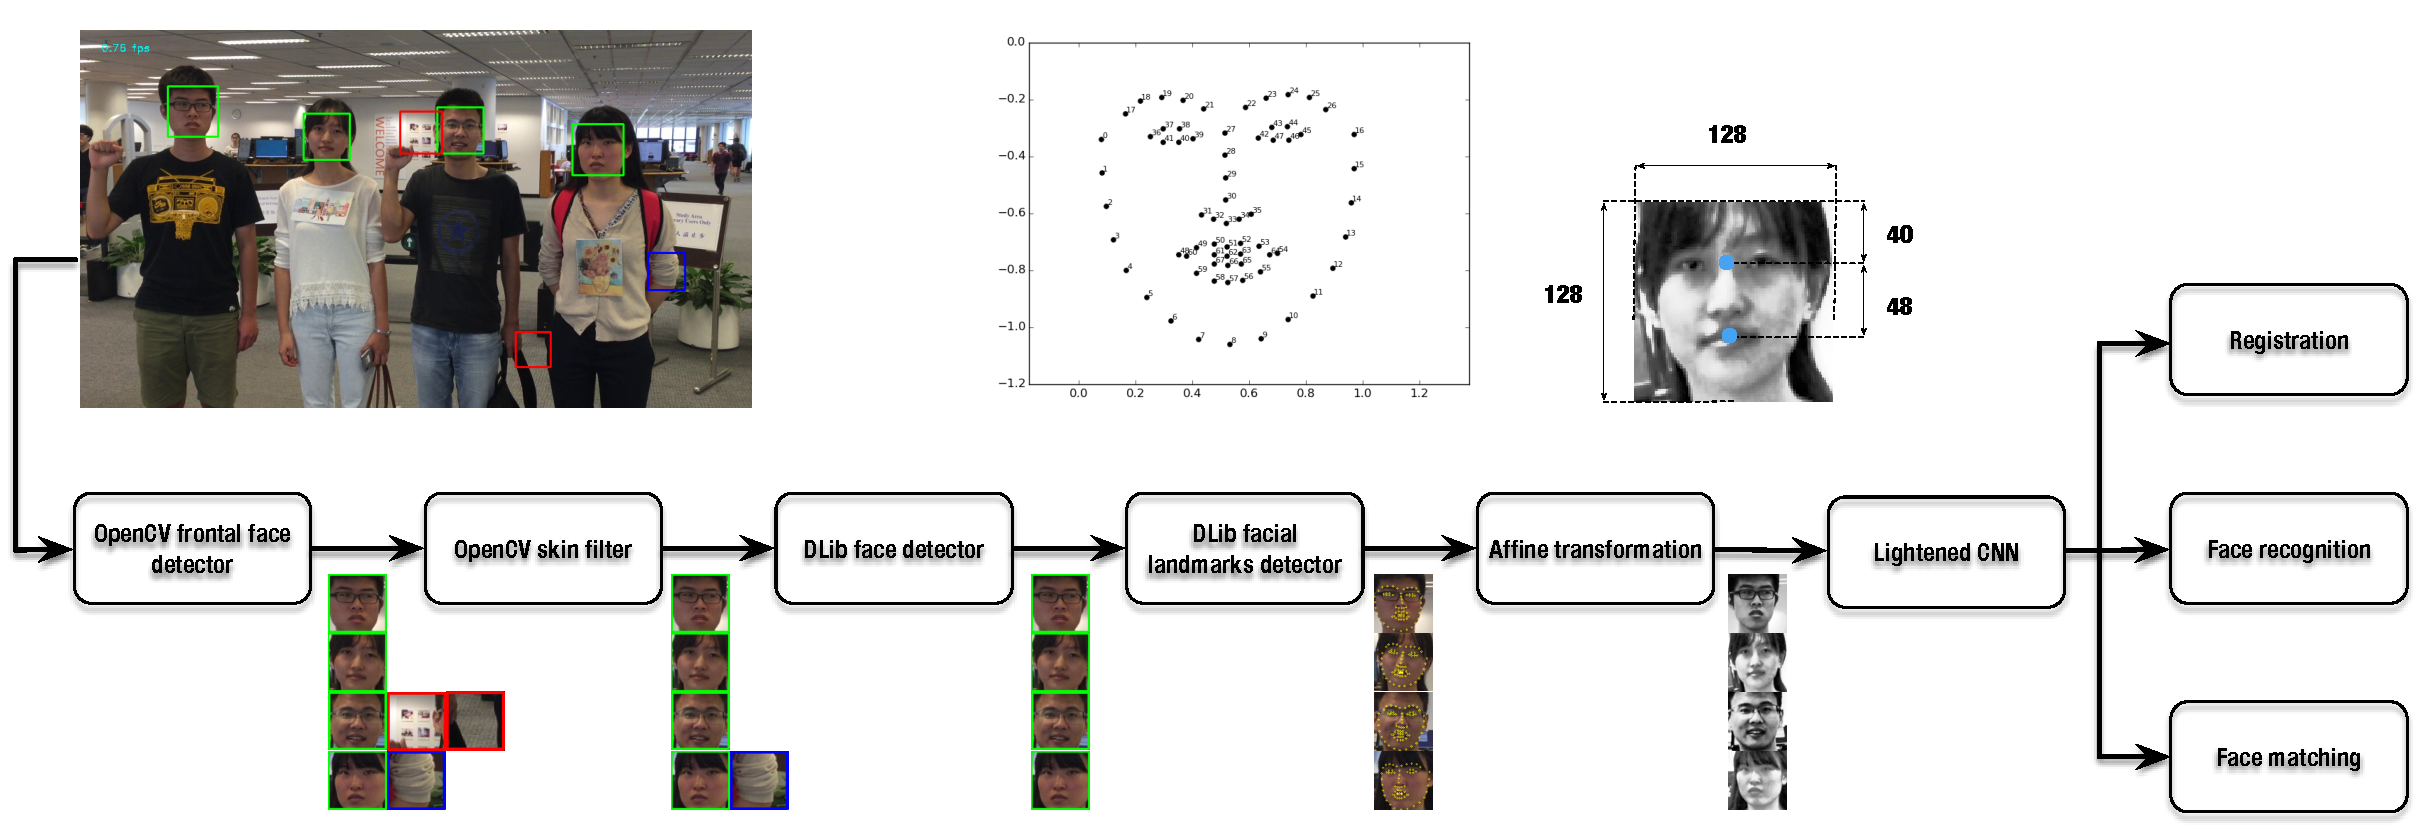
\includegraphics[width=1.0\textwidth]{figure/ch4-facedetalign.pdf}
    \caption{Face detection and alignment workflow.}
    \label{fig:ch4-facedetalign}
\end{figure}

\subsubsection{Recognition}
All the facial features uploaded by registered users are used to train a classifier in the cloud server, using LIBSVM library~\cite{chang2011libsvm}. During training, we set the parameter to enable probability estimations of classes $p_i, i\in{1, \cdots, N}$. In prediction time for each facial feature, if $\max_ip_i \leq 0.3$, then we treat it as from an unknown person who hasn't registered in Cardea, otherwise it is from the user who has the highest probability and his privacy preference will be fetched for further processing.

\subsubsection{Matching}
Face matching occurs when a recognized user $A$ has also specified and uploaded features of person $B$ with whom he doesn't want to be captured, it is to determine whether $B$ also appears in this captured image. Note that $B$ is not necessarily a registered user of Cardea. It is required that $N_B$, the number of $B$'s facial features uploaded by $A$ should be more than $10$. Then feature $f_l$ from other faces $l\neq A$ in the image will be compared with $B$'s features. $\mathtt{Cosine}$ similarity is used as distance metric. Among $N_B$ distances between $f_l$ and $B$'s features, we can calculate the ratio $r$ of distances which are shorter than a threshold $d_ \mathit{threshold}$, if the ratio $r$ is higher than a threshold $r_ \mathit{threshold}$, then $l$ and $B$ are the same person, thus $B$ appears with $A$ in the same image. By tuning, we find $d_ \mathit{threshold} \in (0.3, 0.5)$ and $r_ \mathit{threshold} \in (0.5, 0.8) $ shows good enough performance. In Fig~\ref{fig:ch4-mfmsim}, we plot the distribution of distance between same person's Lightened CNN features and different person's Lightened CNN features. The features are extracted from all the faces in ORL face database~\cite{links:orlfacedb}, which consists of 400 images from 40 distinct subjects, 10 images per subject. Each subject has different photos, such as: with/without glasses, open/closed eyes, and different facial expressions. It is obviously seen that distances between same person and different persons are well seprated, especially for the case of $\mathtt{cosine}$ similarity.

\begin{figure}[!htbp]
    \centering
    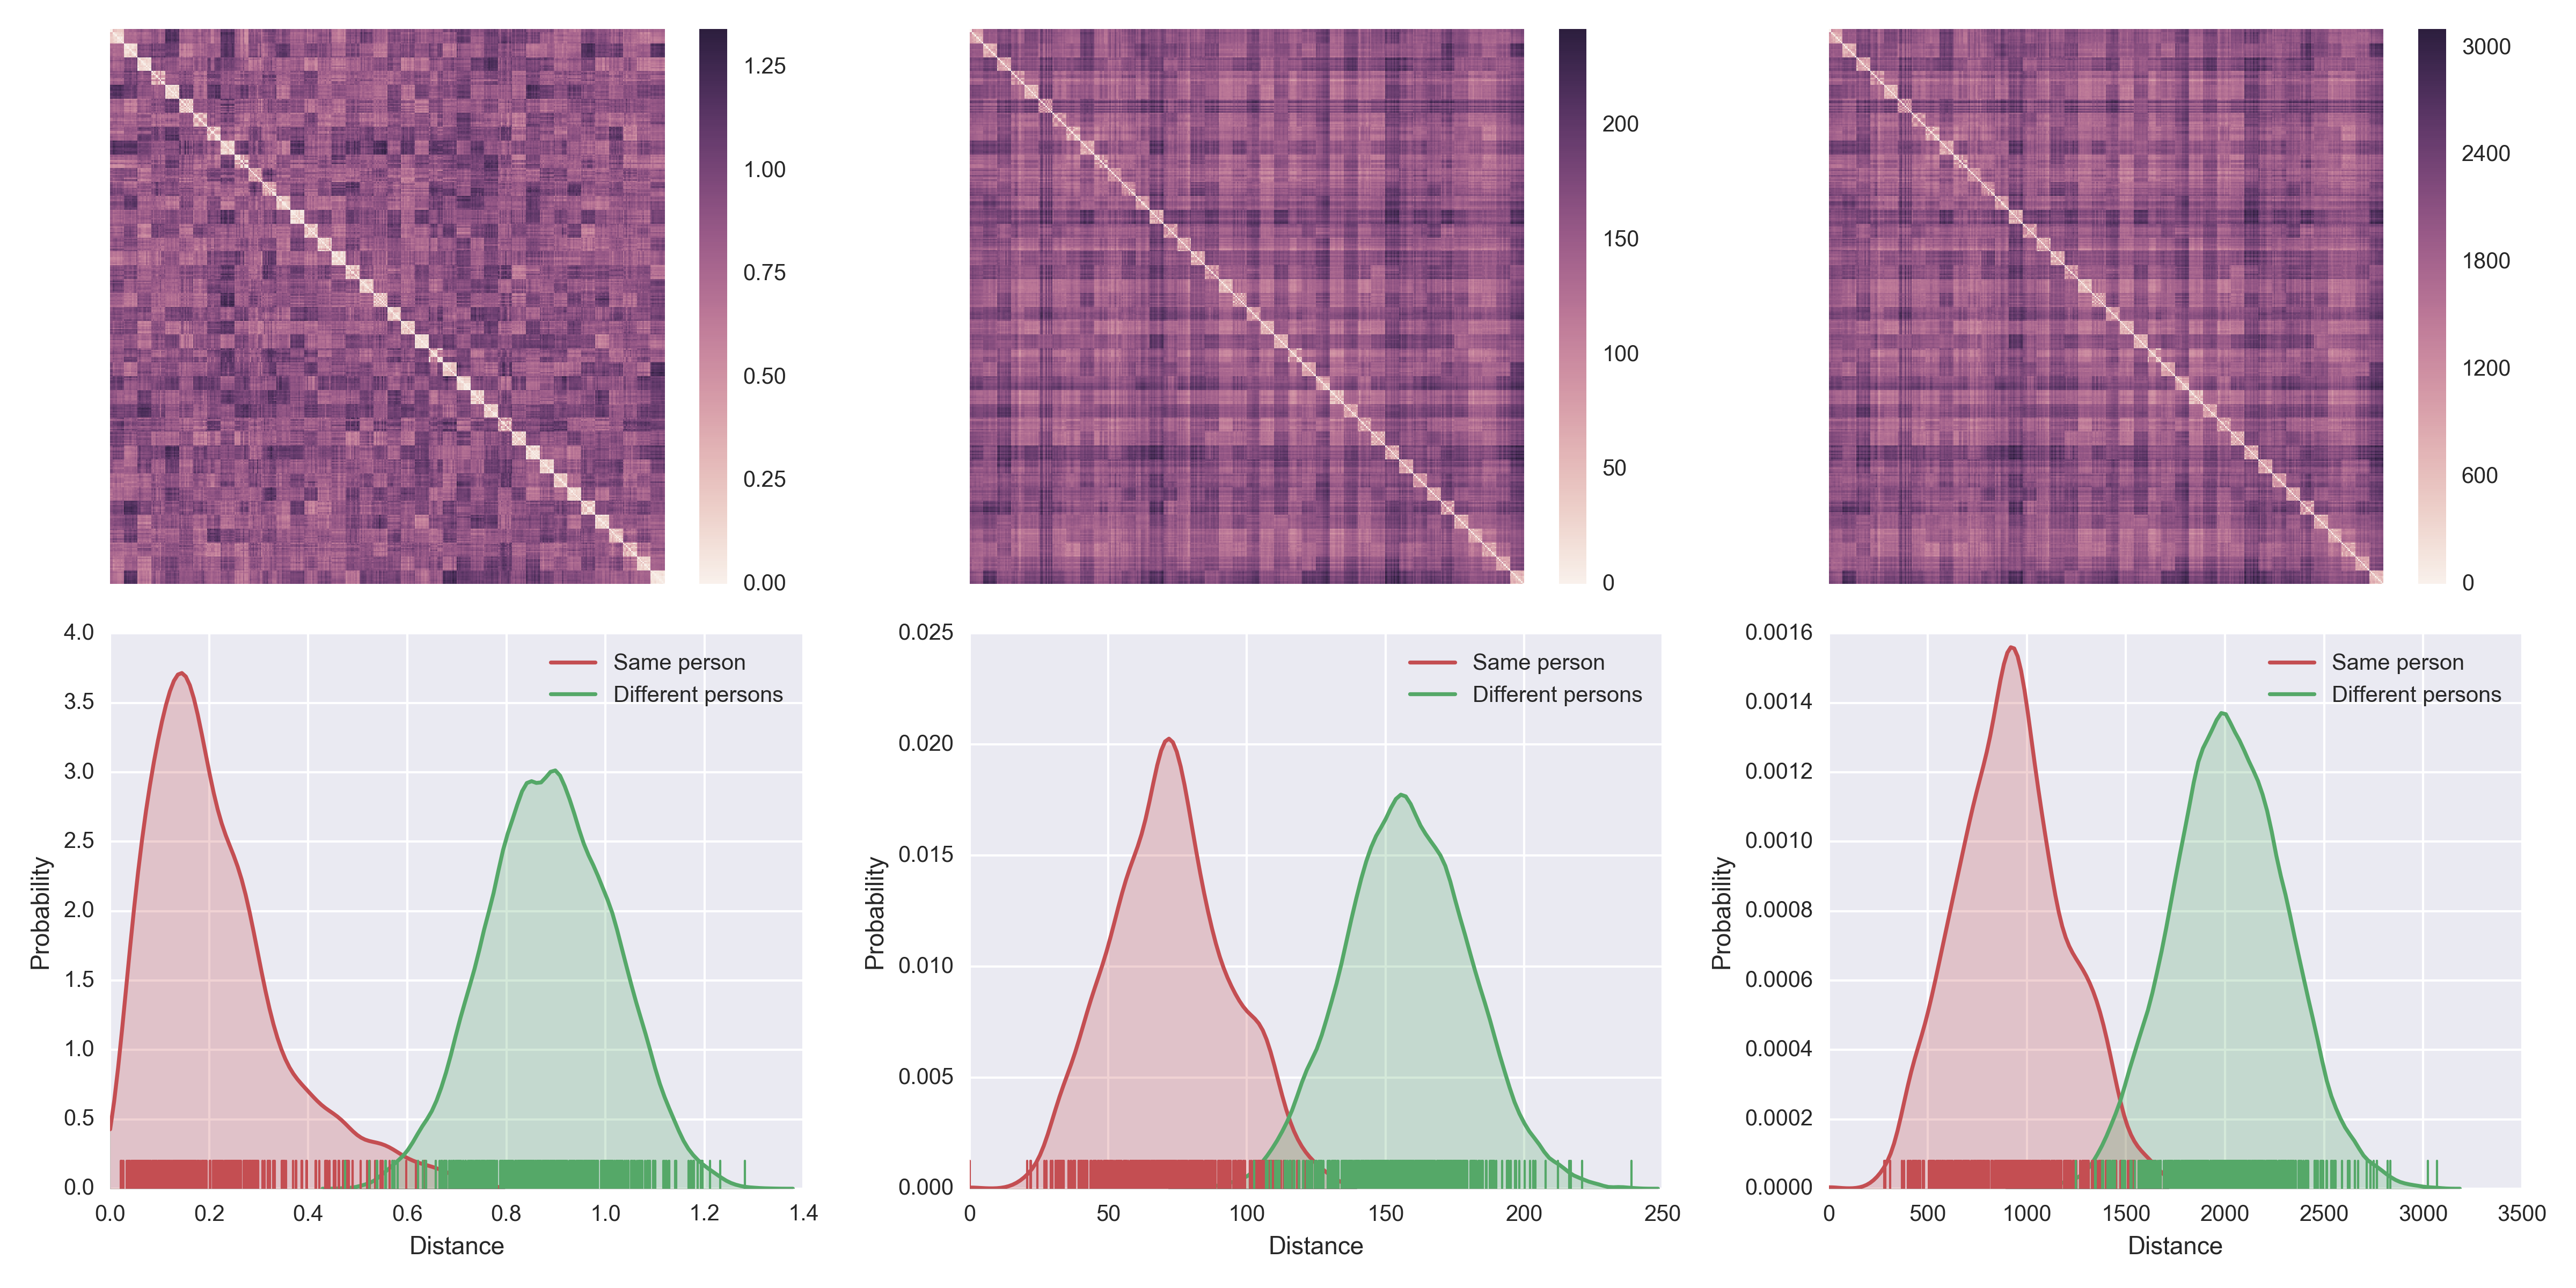
\includegraphics[width=1.0\textwidth]{figure/ch4-mfmsim.png}
    \caption{Distance matrix (top) and distance distribution (bottom) of Lightened CNN features using $\mathtt{cosine}$ similarity (left), $l_1$ norm (center) and $l_2$ norm.}
    \label{fig:ch4-mfmsim}
\end{figure}


\subsection{Gesture Recognition}
In Cardea, "yes" (\vcenteredinclude{figure/ch4-yesgesticon.png}) and "no" (\vcenteredinclude{figure/ch4-nogesticon.png}) gestures have the highest priorities and are used to temporarily overwrite privacy preferences. To recognize gestures in daily life images, the first step is detection of hands, and it turns out to be the most challenging part in this sub task. Skin color based hand detector will fail dramatically in images with cluttered background. A much more robust method will be using multiple proposals~\cite{mittal2011hand} based on hand shape, context, and skin color. However, it takes an extremely long time to detect hands in one image. Finally, we choose to leverage state-of-the-art detection framework faster R-CNN~\cite{ren2015faster} to train a gesture detector in an end-to-end manner.

\subsubsection{Data Preparing and Preprocessing}


VGG group has shared a comprehensive dataset of hand images collected from various different public image data set sources in~\cite{mittal2011hand, links:vgghanddataset}. It contains 5628 images, which is composed of 4069 training images, 738 validation images, 821 testing images respectively, each image is with annotations of hand bounding boxes. However, this dataset can only let us train a hand detector. To achieve the goal of recognizing gestures, there are two solutions in our consideration:

\begin{itemize}
\item First train a hand detector using this dataset, then train another hand gesture classifier using other commonly used gesture datasets and pipe them together.
\item Take this dataset as a subset of images with "normal" gestures, then prepare extra images with "yes" and "no" gestures including annotations by ourselves, and train a "normal/yes/no" gesture detector end-to-end.
\end{itemize}

The first solution is not an end-to-end solution, and the specific "yes" and "no" gestures may not be included in those standard gesture datasets, then we will still need to prepare our specific gesture dataset like in second solution. Therefore, we choose the second solution, based on the observation and also assumption that annotated hands in VGG's hand dataset are in normal relaxing modes, thus will not be treated as "yes" or "no" gestures. The annotations of VGG dataset are tilted rectangles shown as yellow ones in Fig~\ref{fig:ch4-gesturedataset}, we re-annotate the dataset using bounding boxes of the original annotations shown as blue rectangles.

We crawled 527 images with "yes" hand gestures, and 363 images with "no" hand gestures. Note that in a crawled image, it may contain different types of hand gestures as shown in Fig~\ref{fig:ch4-gesturedataset}, which is not a problem so long as gesture types are annotated correctly (\emph{remind} that all gestures in VGG dataset are treated as "normal" class). These images are crawled from Google and Flickr image search with keywords such as "victory sign", "stop gesture", "palm gesture" and so on, many of them are focused on the hands thus don't contain many background pixels. We rescale these images in different scales and then pad zeros on rescaled images. In Faster-RCNN python implementation~\cite{links:pyfasterrcnn}, an input image is rescaled to around $1000\times 1000$ before fed to region proposal network. If without padding data augmentation step, the bounding boxes of hand gestures will be huge in many crawled images that are focused on hands, which makes the learned model not able to detect small hand gestures and also not perform well on the regression of large hand gestures. Another reason for the padding step is to counter data imbalance of three classes. After augmentation, we have a dataset of 13843 images, including 5628 images from VGG dataset, 4712 augmented images mostly with "yes" gestures and 3503 augmented images mostly with "no" gestures. Fig~\ref{fig:ch4-gesturedataset} shows some sample images with annotations from this composed dataset. We wrote a tool~\cite{links:imgannota} to annotate the crawled images.

\begin{figure}[!htbp]
    \centering
    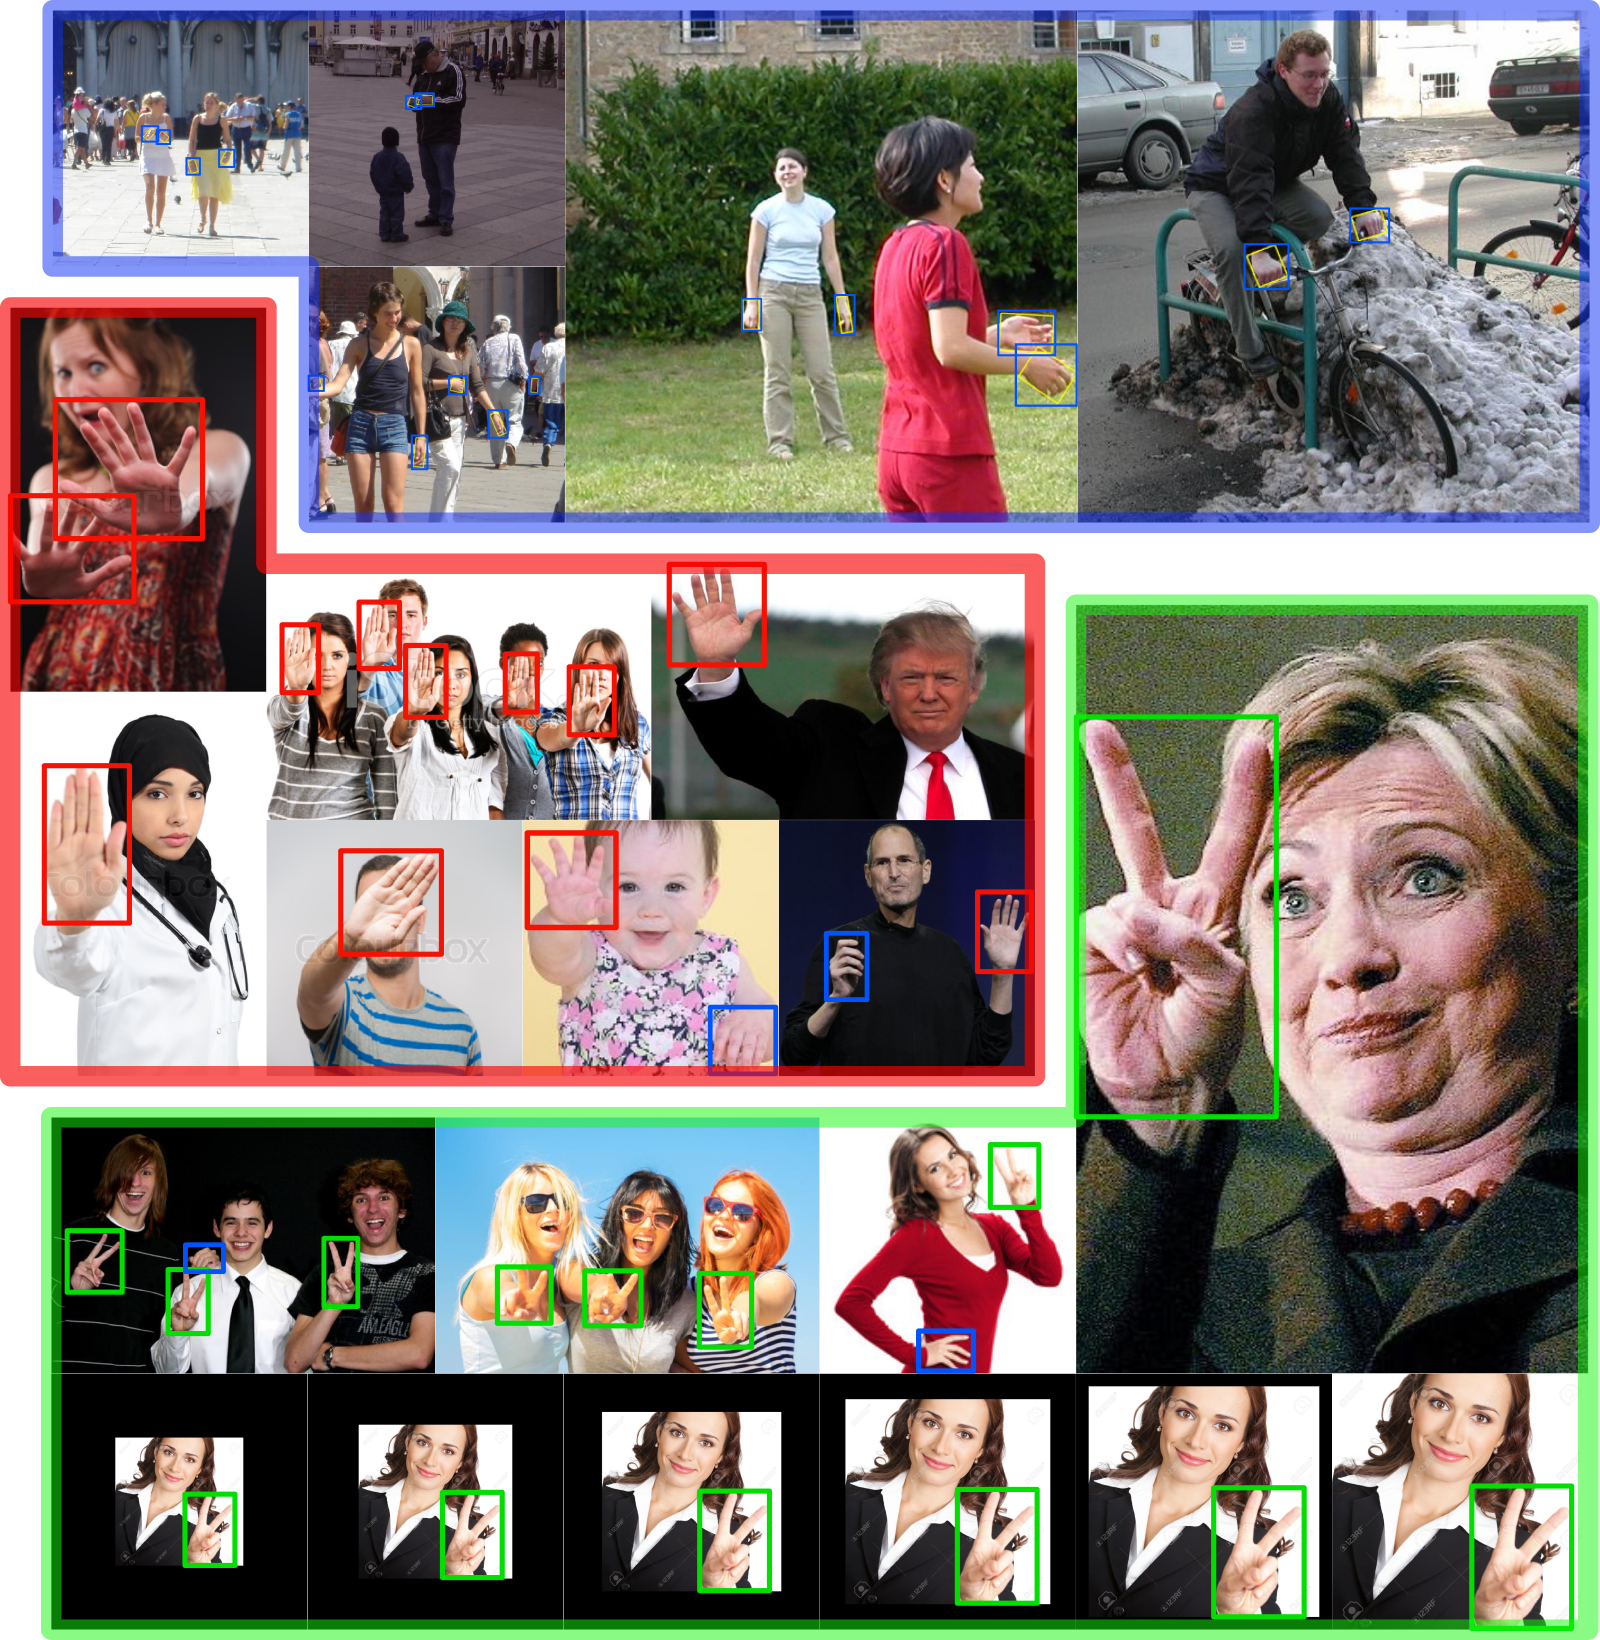
\includegraphics[width=0.8\textwidth]{figure/ch4-gesturedataset.png}
    \caption{Training hand gesture dataset composed of VGG hand dataset (blue) and augmented crawled dataset (red and green).}
    \label{fig:ch4-gesturedataset}
\end{figure}

\subsubsection{Training Procedures}
Using the composed dataset, we fine-tune the \emph{conv3\_1} and up layers of VGG16 pre-trained model provided by Faster-RCNN library, jointly with region proposal layers and detection layers that are not part of VGG16 pre-trained model. Features from \emph{conv5\_3} layer of VGG16 network are shared by region proposal network (RPN) and Fast-RCNN~\cite{girshick2015fast} detection network, RPN uses them to generate proposals, and region of interest (ROI) pooling layer in detecting network uses them for bounding box regression and classification. There are two methods to train a shared feature extraction network. One is an alternating optimization method with following steps: \ding{182} Train an RPN $M_1$ initialized from VGG16 pre-trained model $M_0$, \ding{183} Generate training proposals $P_1$ using RPN $M_1$, \ding{184} Train Fast R-CNN model $M_2$ on proposals $P_1$ initialized from $M_0$, \ding{185} Train RPN $M_3$ from $M_2$ without changing convolutional layers, \ding{186} Generating proposals $P_2$ using RPN $M_2$, \ding{187} Train Fast R-CNN model $M_4$ on proposals $P_2$ initialized from $M_3$ without changing convolutional layers, \ding{187} Add $M_3$'s RPN layers to Fast R-CNN model $P_2$. Another method is an approximate joint optimization method by training with stochastic gradient descent as usual, which is easier, faster and achieves similar performance~\cite{links:pyfasterrcnn}, so we use the second training procedures.

\subsubsection{Prediction}




\subsection{Deployment on Android}

Ideally, for a privacy control framework, we prefer a design that does not require cloud server and all the algorithms run locally on mobile devices. In the current design and implementation, cloud server exists mainly for two reasons: \ding{182} Storage center for profiles and hosting face recognition model; \ding{183} RPN in gesture recognition task is written in Python language, thus gesture recognition can not run on Android smartphones easily. However, these are not hard restrictions, possible improvements are discussed in Chapter 5.

The deployment of Caffe models for scene classification and facial feature extraction is based on Caffe-android-library~\cite{links:caffeandroidlib}, we modified its code~\cite{links:caffeandroidlibzr} to support loading multiple Caffe models, batch feature extraction, and only forwarding to a specified layer during feature extraction, which saves useless computations from fully connected layers. The deployed scene classification model (based on AlexNet structure) has a size of 230MB, which is not small. However, its prediction is very fast, and can be easily fitted into the time slot of waiting response from cloud server. The facial feature extraction model (based on Lightened CNN structure) has a relatively bearable size of 33MB. Comparing to AlexNet, Lightened CNN model has smaller filter sizes, but with many more feature maps, therefore in run time, Lightened CNN model consumes about 1GB memory, which makes it not able to run on smartphones with less than 2GB memory~\ref{tbl-forwardingtime}. Possible ways to decrease model size and optimization of resource consumptions are also discussed in next chapter. Other lighter models we deployed on android include OpenCV face cascading model (less than 1MB), and shape predictor (90MB) in Dlib facial landmark detection.


\subsection{System Integration}

\begin{figure}[!htbp]
    \centering
    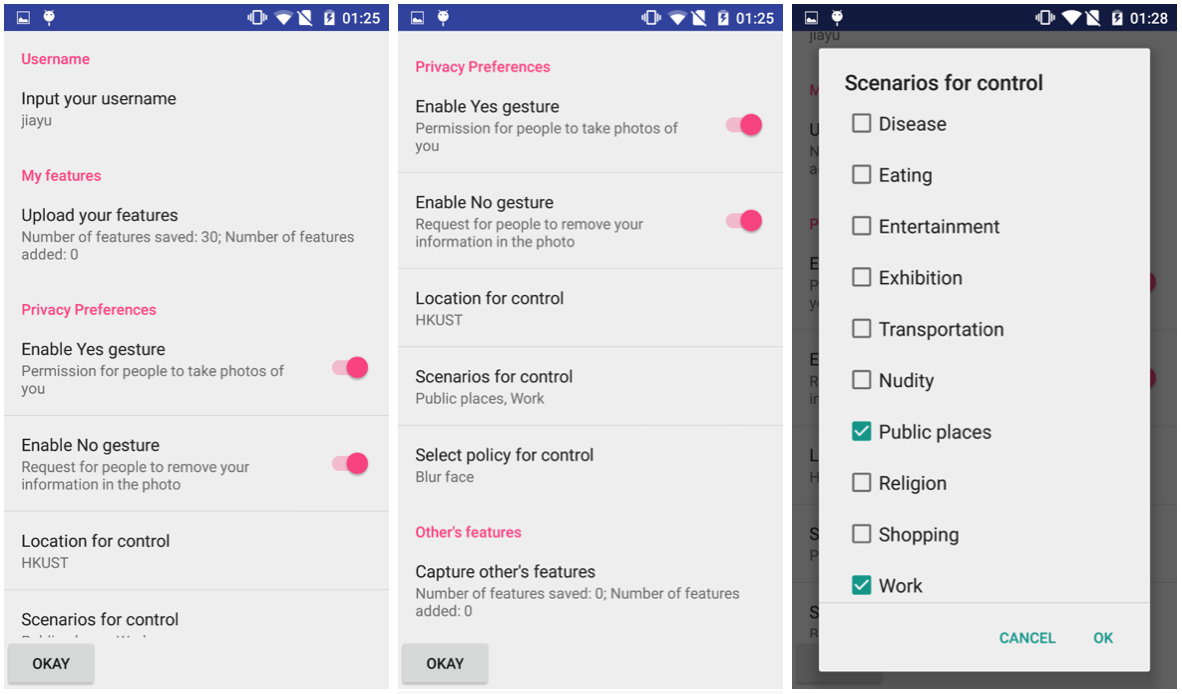
\includegraphics[width=0.8\textwidth]{figure/ch4-reg.png}
    \caption{Registration interface}
    \label{fig:ch4-reg}
\end{figure}

Fig~\ref{fig:ch4-cardeadataflow} gives the dataflow of Cardea:


\begin{description}[leftmargin=0cm]
  \item[{Registration}] The interface of registration for bystanders is shown in Fig~\ref{fig:ch4-reg}


\end{description}


\begin{figure}[!htbp]
    \centering
    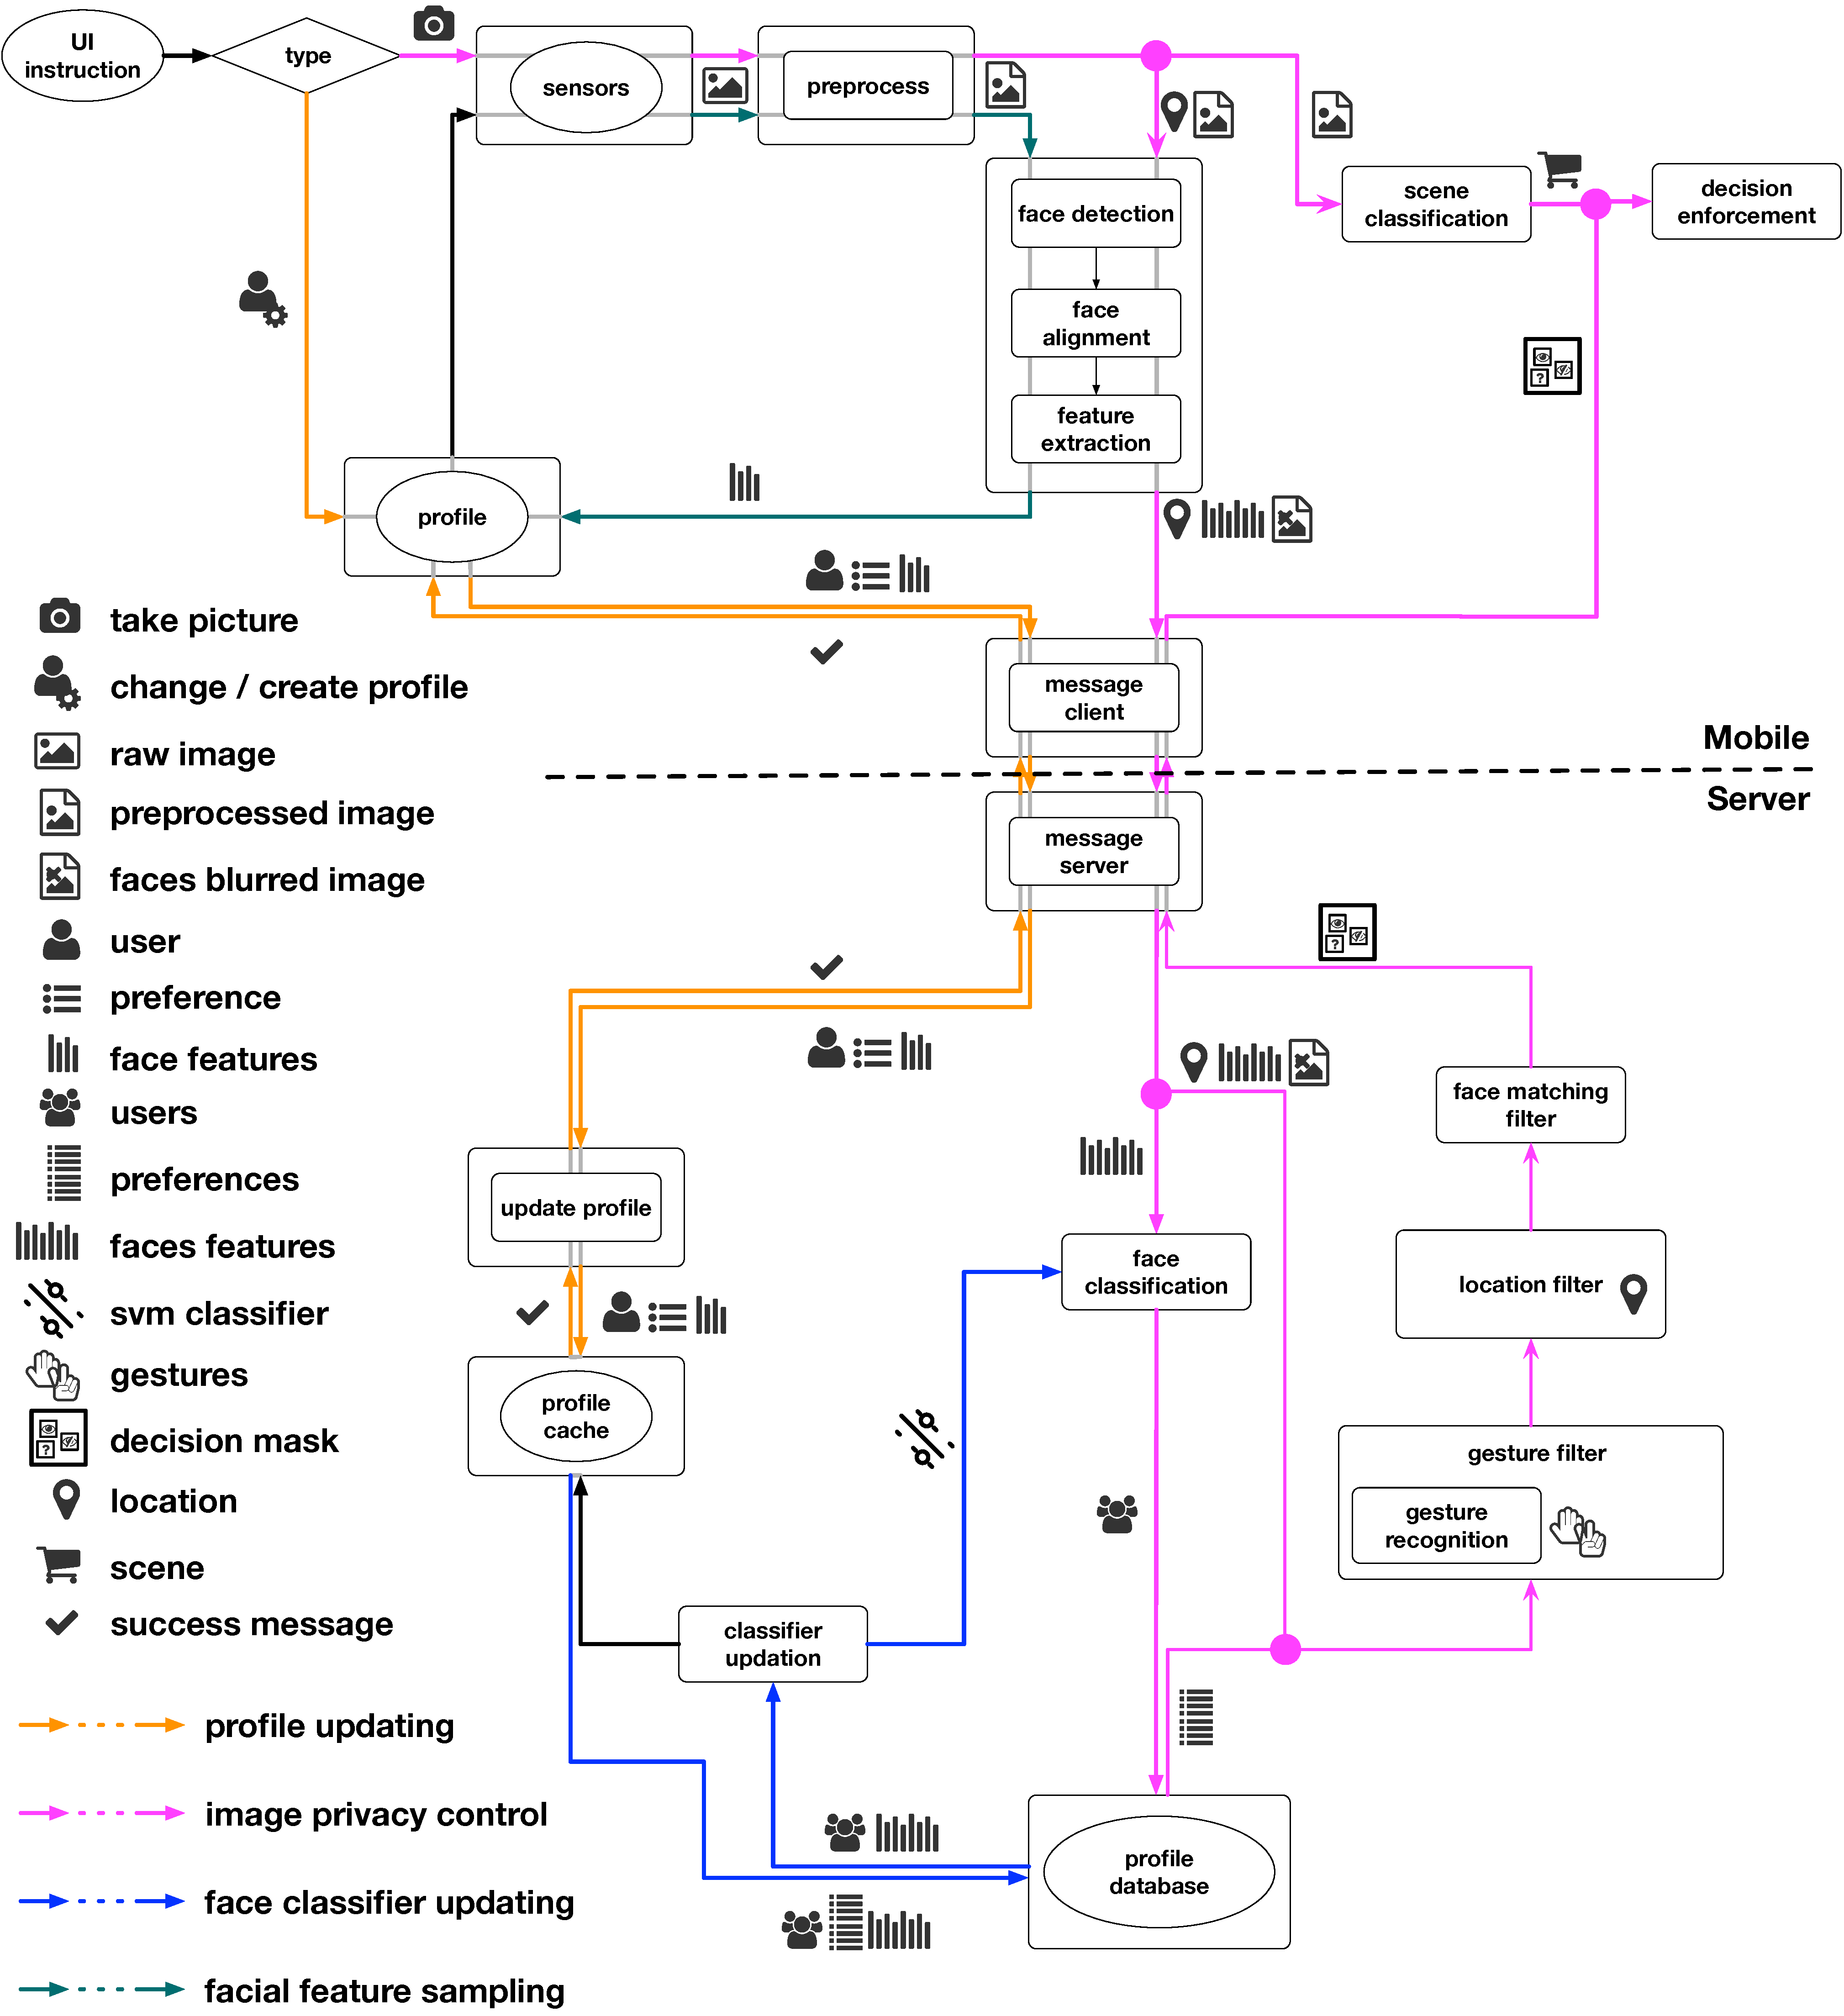
\includegraphics[width=0.8\textwidth]{figure/ch4-cardeadataflow.pdf}
    \caption{Dataflow of Cardea}
    \label{fig:ch4-cardeadataflow}
\end{figure}
message package header

screen shots

decision tree



The implementation of Cardea is hosted in~\cite{links:cardeaproj}.

\section{Evaluation}


\newpage
